%---------------------------------------------------------------------
%			Preamble
%---------------------------------------------------------------------

% This thesis template has been prepared by:

	% Monika Bialy
	% Department of Computing and Software
	% Faculty of Engineering
	% McMaster University
	% 1280 Main St W, Hamilton, ON L8S 4L8
	% bialym2@mcmaster.ca


% Formatting of this document conforms to the "Guide for the Preparation of Master's and Doctoral Theses" as defined by McMaster University's School of Graduate Studies. The aforementioned guide may be found at http://graduate.mcmaster.ca/images/2014_uploads/Guide_for_the_Preparation_of_Theses_May2014.pdf

% 2015-07-23: Fixed DescriptiveNote TOC link and removed supefluous options - Alexander Schaap
% 2019-01-29: Updated with the latest requirements from the 2016 version of the guide (https://gs.mcmaster.ca/sites/default/files/resources/guide_for_the_preparation_of_masters_and_doctoral_theses-_december_2016.pdf) - Syed Asim Shah

%---------------------------------------------------------------------

\documentclass[12pt, oneside]{book}

\setcounter{secnumdepth}{3}	% Make sub subsections numbered
\setcounter{tocdepth}{3}

%---------------------------------------------------------------------
%			Packages
%---------------------------------------------------------------------

% -- For Formatting --
%For students who wish to send a copy  (or  copies)  of  their  finally-approved thesis  for  binding,  the  following should be noted. To ensure sufficient space on the page for  binding,  the  TOP and LEFT margins  should  be 3.8 cm, and the RIGHT and BOTTOM margins should be 2.5 cm. If the thesis is to be back printed, both LEFT and RIGHT margins should be 3.8 cm. These margins also apply to all illustrative material, including diagrams, maps, photographs, charts, tables, and computer printouts.
\usepackage[top=3.8cm, bottom=2.5cm, left=3.8cm, right=3.8cm]{geometry}
\usepackage{setspace}	% For changing the line spacing. Already included for the markup, so commented out for now
\usepackage{xspace}
\usepackage{fancyhdr}
\usepackage[nottoc]{tocbibind}	%  Adds bib, list of figs, and list of tables to the table of contents
\usepackage[linktocpage, colorlinks, linkcolor=blue, citecolor=blue]{hyperref}	% Links page numbers to their pages, and include page nuns in bib
\usepackage[printonlyused,withpage]{acronym} 
\usepackage[toc,page]{appendix}
\usepackage{booktabs}
\usepackage{csquotes}
\usepackage{array}
\usepackage{longtable}
\usepackage{rotating}
\usepackage[tableposition=t]{caption}


% -- For Bibliography --
\usepackage[style=numeric, sorting=none, backend=bibtex, backref, doi=false]{biblatex}	% Use Biblatex for customization of bib
\addbibresource{Thesis.bib}

% -- For Figures --
\usepackage{graphicx}
\graphicspath{{Figures/}}
\usepackage{float}
\usepackage{svg}
\svgpath{{Figures/}}
\usepackage{pdfpages}
\usepackage{listings}

\lstset{frame=tb,
	language=Java,
	aboveskip=3mm,
	belowskip=3mm,
	showstringspaces=false,
	columns=flexible,
	basicstyle={\small\ttfamily},
	numbers=none,
	numberstyle=\tiny\color{gray},
	keywordstyle=\color{blue},
	commentstyle=\color{dkgreen},
	stringstyle=\color{purple},
	breaklines=true,
	breakatwhitespace=true,
	tabsize=3,
	upquote=false
}


% -- For Math --
\usepackage{amsmath}
\usepackage{amssymb}
\usepackage{tipa}
\usepackage{cleveref}


%---------------------------------------------------------------------
%			 Hacks 
%---------------------------------------------------------------------

% -- Make citation author names link to bibliography entry. Biblatex only does year links by default --
\DeclareFieldFormat{citehyperref}{%
  \DeclareFieldAlias{bibhyperref}{noformat}% Avoid nested links
  \bibhyperref{#1}}

\DeclareFieldFormat{textcitehyperref}{%
  \DeclareFieldAlias{bibhyperref}{noformat}% Avoid nested links
  \bibhyperref{%
    #1%
    \ifbool{cbx:parens}
      {\bibcloseparen\global\boolfalse{cbx:parens}}
      {}}}

\savebibmacro{cite}
\savebibmacro{textcite}

\renewbibmacro*{cite}{%
  \printtext[citehyperref]{%
    \restorebibmacro{cite}%
    \usebibmacro{cite}}}

\renewbibmacro*{textcite}{%
  \ifboolexpr{
    ( not test {\iffieldundef{prenote}} and
      test {\ifnumequal{\value{citecount}}{1}} )
    or
    ( not test {\iffieldundef{postnote}} and
      test {\ifnumequal{\value{citecount}}{\value{citetotal}}} )
  }
    {\DeclareFieldAlias{textcitehyperref}{noformat}}
    {}%
  \printtext[textcitehyperref]{%
    \restorebibmacro{textcite}%
    \usebibmacro{textcite}}}
    
% -- Remove colour of acronym hyperlinks --
\makeatletter
\AtBeginDocument{%
  \renewcommand*{\AC@hyperlink}[2]{%
    \begingroup
      \hypersetup{hidelinks}%
      \hyperlink{#1}{#2}%
    \endgroup
  }%
}
\makeatother
 
%---------------------------------------------------------------------
%		     Macros for Writing
%---------------------------------------------------------------------

\newcommand{\ThesisTitle}{CyclicL - An Approach to Automated Requirement Traceability in Product Line Engineering}
\newcommand{\Author}{Thomas Chiang}
\newcommand{\Supervisors}{Richard Paige, Alan Wassyng}
\newcommand{\DegreeName}{PhD}
\newcommand{\DegreeAbbr}{PhD}
\newcommand{\PastDegrees}{B.Eng Computer Engineering, M.A.Sc Software Engineering}
\newcommand{\PastUniversity}{McMaster University}
\newcommand{\UniversityName}{McMaster University}
\newcommand{\UniversityDept}{Computing and Software}
\newcommand{\MonthYearOfSubmission}{Jan, 2021}
\newcommand{\FigureLoc}{}

\newcommand{\tool}{CyclicL}
\newcommand{\pgd}{PG\_Device}





%---------------------------------------------------------------------
%			 Document 
%---------------------------------------------------------------------

\begin{document}

%---------------------------------------------------------------------
%			Frontmatter
%---------------------------------------------------------------------

\frontmatter   
\doublespacing
	
	\begin{titlepage}
\begin{center}

	\vspace*{3cm}
	
	{\LARGE \textsc{\ThesisTitle} \par}
	
	\vspace{2.5cm}
	
	By \\
	\vspace*{.25cm}
	
	{\large \textsc{\Author}}
	
	\vspace{2.5cm}
	
	A Thesis \vskip .2cm Submitted to the School of Graduate Studies \\  in Partial Fulfillment of the Requirements for the Degree \vskip .2cm\DegreeName
	
	\vfill
	
	\UniversityName \\
	 \copyright ~Copyright by Thomas Chiang, \MonthYearOfSubmission

\end{center}
\end{titlepage}







	
	\setcounter{page}{2}
	\pagestyle{plain}
	
	\phantomsection % Enable TOC to link to this page as one expects
\begin{tabbing}
	\textsc{\DegreeName} (\MonthYearOfSubmission) \hspace{3cm}	\= \UniversityName		\\
	(Software Engineering)			 	\> Hamilton, Ontario	\\[1cm]
\end{tabbing}

\noindent\begin{tabular}{l p{.73\textwidth}}
	\textsc{Title:} 		& \ThesisTitle 						\\[.6cm]
	\textsc{Author:} 		& \Author, \PastDegrees ~(\PastUniversity) 		\\[.6cm]
	\textsc{Supervisors:} 	& \Supervisors			 			\\[.6cm]
	\textsc{Number of Pages:} & \pageref{ContentStart}, \pageref{ContentEnd} 	\\[.6cm]
\end{tabular}
	\addcontentsline{toc}{chapter}{Descriptive Note}	% DONE: This line now links correctly (\phantomsection)

	\chapter*{Lay Abstract}

%A lay abstract of not more 150 words must be included explaining the key goals and contributions of the thesis in lay terms that is accessible to the general public. This page must be numbered ‘iii’.
The purpose of this paper is to 
	\addcontentsline{toc}{chapter}{Lay Abstract}
	
	\chapter*{Abstract}

%An abstract of not more than 300 words must be included and will indicate the major emphasis of the thesis, new discoveries, and its contribution to knowledge.
\ac{PLE} has become a common engineering practice for managing system complexity across multiple industries. The practice is used for identifying reusable pieces of code, composing software components together, and modelling product variation. There exists a gap however with generating system traceability when using \ac{PLE} as a technique. Specifically, it is a colossal problem to get traceability from a feature model, the modelling environment for \ac{PLE}, through requirements to design elements. Further, traceability itself is both a costly and tedious task that is often completed at the end of development and even more difficult to maintain throughout a products life-cycle. With the methodology proposed in this thesis, along with its supporting tool \tool, we aim to address the gap that exists between \ac{PLE} and requirement engineering to push traceability out of a retrospective task to an active portion of development.
	\addcontentsline{toc}{chapter}{Abstract}

	\chapter*{Acknowledgments}

An expression of thanks to supervisors, industry partners, colleagues, family, or friends.
	\addcontentsline{toc}{chapter}{Acknowledgments}


	
\onehalfspacing
	\tableofcontents
	\addcontentsline{toc}{chapter}{Table of Contents}
	\label{ContentStart}	% Denotes where the thesis content starts, i.e. after the table of contents

	\listoffigures
	
	\listoftables
	
	\clearpage
	
	\section*{List of Acronyms}
	\addcontentsline{toc}{chapter}{List of Acronyms}
		\begin{acronym}
			\acro{MDE}[MDE]{Model-Driven Engineering}
			\acro{EMF}[EMF]{Eclipse Modeling Framework}
			\acro{DSL}[DSL]{Domain Specific Language}
			\acro{EOL}[EOL]{Epsilon Object Language}
			\acro{MOF}[MOF]{Meta-Object Facility}
			\acro{OMG}[OMG]{Object Management Group}
			\acro{OCL}[OCL]{Object Constraint Language}
			\acro{ETL}[ETL]{Epsilon Transformation Language}
			\acro{EML}[EML]{Epsilon Merging Language}
			\acro{GMF}[GMF]{Graphical Modeling Framework}
			\acro{DSM}[DSM]{Domain Specific Model}
			\acro{PLE}[PLE]{Product Line Engineering}
			\acro{CIA}[CIA]{Change Impact Anlaysis}
			\acro{FDD}[FDD]{Feature-Driven Development}
			\acro{FODA}[FODA]{Feature-Oriented Domain Analysis}
			\acro{FORM}[FORM]{Feature-Oriented Reuse Method}
			\acro{UCD}[UCD]{Use Case Diagram}
			\acro{ACC}[ACC]{Adaptive Cruise Control}
			\acro{AQL}[AQL]{Acceleo Querying Language}
			\acro{EVL}[EVL]{Eclipse Validation Language}
			%Define acronyms here
			%Use intext with \ac{}. Look at reference for the acronym package for a full guide
		\end{acronym}

	\chapter*{Declaration of \\Academic Achievement}

The student will declare his/her research contribution and, as appropriate, those of colleagues or other contributors to the contents of the thesis.
	\addcontentsline{toc}{chapter}{Declaration of Academic Achievement}

	\clearpage

%---------------------------------------------------------------------
%			Mainmatter
%---------------------------------------------------------------------
\mainmatter
\doublespacing

	%---------------------------------------------------------------------
	%		Custom headers/footers for mainmatter
	%---------------------------------------------------------------------
	
	\fancypagestyle{fancyplain}{
		\fancyhf{}
		\fancyfoot[C]{\thepage}
		\fancyhead[L]{\footnotesize \DegreeAbbr~ Thesis -- \Author}
		\fancyhead[R]{\footnotesize   \UniversityName~-- \UniversityDept}
	}
	\pagestyle{fancyplain}	% Use fancyplain style henceforth

	\fancypagestyle{plain}{ 	% Redefinition of plain for the chapter pages
		\fancyhf{}
		\fancyfoot[C]{\thepage}
		\fancyhead[L]{\footnotesize \DegreeAbbr~ Thesis -- \Author}
		\fancyhead[R]{\footnotesize   \UniversityName~-- \UniversityDept}
	}
	%---------------------------------------------------------------------
	\chapter{Introduction}

What came first, the chicken or the egg? It is a silly question that people will often debate about over dinner or on the bus. In engineering there is a similar debate; what comes first, the feature or the requirement? Very often when we do engineering work we consider what we want to build in parallel to actually thinking about building it; exploring the problem space often gets overlooked in favor of exploring the solution space. As a result, an engineer may have to reflect on their requirements when they hit a wall during development. They may find that their requirements were incomplete for their feature. Perhaps the scope of their feature is much bigger than they anticipated; maybe what was originally considered to be a single feature could in fact be multiple features. Thus, the engineer will iterate back and forth between feature development and requirement development, incrementally changing each until they get to a system state that they consider to be complete, or at the very least a minimum viable product. 

How do we capture this process? \ac{FDD}~\cite{palmer2001practical} is a common method for agile development whereby the engineers will identify a set of features that will be built together to create a system, often leveraging \ac{MDE} techniques as well. They will then work to identify acceptance criteria, or descriptions of each feature to specify what needs to be done for each feature and how to know when it is complete. These descriptions end up serving a similar role as requirements for the features, if not outright being written as requirements for the feature. Therefore, we can make the proposition that before we have requirements, we have features. The features come first, thus we should focus on identifying features before we start to think about what requirements we need for a given system. This situation will often arise when a new product is being developed, or a company is just starting up.

There is an unusual assumption made in this scenario; are there not already existing requirements before we begin to identify features? From another perspective, in more mature development teams and industries it is uncommon to start from scratch without any requirements, and even more rare to jump right into identifying solutions without first having an idea of what the problems are. Thus, even if limited, there are at least some guiding requirements before engineers begin to identify features of their system that will solve their problems. Therefore, we can say that requirement come before the features. In this environment, we already have a rich history to pull from to help inform any new development that may come up.

In reality, both scenarios are likely to happen, perhaps even within the same company! Innovation in industry is constant and there are always new products being developed both from scratch or iteratively on existing products. We may be able to pull from existing assets from one product to help with the development of an entirely new product. Conversely, we may be branching off into an entirely new domain with no existing documentation or reusable assets. Thus we have to start from scratch at understanding what problems exist within the new domain. Both scenarios are equally valid!

%In reality, both scenarios are likely to happen, perhaps even within the same company. We may find that we have a vague idea of what the problem is, perhaps even some simple drafts of the problems and what requirements we may have to solve them. However, it is common that we know what we want to build before we specify anything of the system as we already have some domain knowledge and can predict what problems we will solve with a given solution. Thus we begin to identify features of our solution and later will go to specify our system what requirements apply to our given features.

The conflicting nature of reality generates a couple of problems for development. The relationship between requirements and features becomes ambiguous. In fact, what are the differentiating factors between a feature and requirement? For this thesis, we will follow the definition of a feature from the original work of Kuang et al.~\cite{kang1990feature, kang1998form} for their Feature-Oriented Domain Analysis \ac{FODA} and Feature-Oriented Reuse Method \ac{FORM}. According to their original definition, a feature is "a prominent or distinctive user-visible aspect, quality, or characteristic of a software system or systems." Based on this definition, we could consider that any portion of a system that a user can interface with is viable to become a feature. In fact for the sake of inclusion, we extend this definition to not only be user-visible, but simply an interface, taking into account the multiple different senses that a user can use to interact with our system. This will increase the scope of a feature beyond what is only visible, including sound, touch, smell, and taste. Depending on product scope, this definition could be extended to other subsystems that interface with the targeted product.

What is a requirement? This is well developed and studied topic. To answer, we look to van Lamsweerde~\cite{lamsweerde2009requirements} where he outlines the purpose of requirements engineering is to answer three question; what, why, and who? What is the problem we are trying to solve? Why is it worth solving? Who should be involved in the solution? There are many more requirements engineering approaches and strategies that we can and will use to develop our methodology, however as a base line when understanding what a requirement is it should answer what the problem is that we are solving supported by sound reasoning for why it is worth being solved and who is involved in solving the problem. 

As such, what are the problems we are trying to solve with this thesis? For one, what is the relationship between features and requirements? This is a problem due to ambiguous relationship between them and the different development styles that exist. As there are dependencies between them, setting a definition of the relationship between them may help with both making sure that we elicit and refine requirements that are correct and reasonably complete. At the same time, it can help to ensure that the features we identify are correct and reasonably complete.

Another issue is that iterations between features and requirements do not happen in isolation. There is usually a lot of supporting documentation and software that surrounds and depends on both the requirements and identified features. This is usually expressed through traceability documentation, most commonly in a traceability matrix. However, maintaining a traceability matrix with all the incremental changes that happen between requirements and features is an extremely tedious and time consuming task. For each change it is usually a low return for high effort task, until such a time that the traceability matrix is so out of sync with both the requirements and features that is it no longer usable. One implication of this is that we will need to create an entirely new traceability matrix and thus the cycle continues. Therefore, traceability documentation is a very large problem during iterative and incremental development.

%\ac{FDD} as a development style misses a very key component. How do all the features fit together? This is a problem that is addressed by Product Line Engineering \ac{PLE}. 

We also examine implication for agile development styles. \ac{FDD} is a feature focused development methodology that already has some set rules for implementation. We also want to explore some possibilities that may exist for adoption into existing development approaches. The objective here would be to explore methods for improvement rather than redefining entirely how \ac{FDD} might be implemented, especially tying it in with \ac{MDE} and \ac{PLE} efforts. This is true both at the conceptual level and the tool support level.

Tools like FeatureIDE~\cite{kastner2009featureide, thum2014featureide} which supports feature composition of software artifacts. Or a tool like GEARS~\cite{GEARS} which emphasizes its 3-tiered software product line methodology. There is also formal methods research for \ac{PLE} such as the work of Peter H\"{o}fner et al.~\cite{hofner2006feature,hofner2011algebra}, which created a formal algebra for how to compute product lines and feature models. What these tools lack however is an self-contained way to manage traceability between features and requirements; FeatureIDE focuses on code composition where GEARS is not cohesive. GEARS requires hooking into separate requirements engineering tools and does not have a way to handle requirements independently. Thus we identify a lack of tool support for traceability and iterations between requirements and features as another problem.

Finally, the problem of how we accomplish all of these tasks? What is the process to help make sure the features we identify are correct and sufficiently complete? What is the process to make sure that we identify requirements that are correct and sufficiently complete? How can we be sure that our mappings between requirements and features also make sense? This is another problem as we want to make sure that the mappings between features and requirements are correct and complete for development tasks as much as for assurance purposes. We want developers to be developing the correct features, and we want to be capable of reasoning about those features so that we can develop assurance that properties of our system are true.

%A confounding variable in all of these problems that we have not yet identified \ac{PLE} is usually a \ac{MDE} process

It is important to note that while not mandatory, many \ac{PLE} efforts also use modelling in their approach. There is a lot of cross-pollination that already exists between the two domains. For our purposes, we want to examine these problems through the lens of \ac{MDE} primarily; can we solve these problems using \ac{MDE} techniques and processes? We support \ac{PLE} through \ac{MDE} techniques and processes rather than using modelling as a means to an end.

In summary, these problems lead to the following research questions:
\begin{enumerate}[label=\textbf{RQ.\arabic*}]
%	\item[RQ1: ]\label{RQ:1} How can we improve requirement elicitation and feature identification processes in \ac{FDD}?
%	\item[RQ2: ]\label{RQ:2} How can we improve traceability maintenance between features and requirements?
%	\item[RQ3: ]\label{RQ:3} How can we improve tool support for iterative and incremental development between features and requirements?
%	\item[RQ4: ]\label{RQ:4} How can we leverage \ac{MDE} techniques for domain analysis, problem space exploration, and requirement
	\item \label{RQ1} How can we improve the state of implementation and usability of \ac{FDD}?
	\item \label{RQ2} How can we improve the maintenance and generation of traceability between features and requirements?
	\item \label{RQ3} How can we improve tool support for iterative and incremental development between features and requirements?
	\item \label{RQ4} How can we leverage \ac{MDE} techniques for domain analysis, problem space exploration, and requirement development?
\end{enumerate}


\section{Motivation}

In many industries, we can find companies that have a catalog of products they offer to customers. There are also many industries that focus on safety-critical application development. Some areas where these two categories overlap are the automotive domain and the medical device domain. Within automotive industry, companies offer a range of vehicles customers can choose for purchase. Further, each of the vehicle models on offer can have variants available. These vehicle model variations can be due to aesthetic difference or functional differences. There can also be variations due to where in the world the vehicle is being sold, such as the driver seat location depending on if the country of sale drives on the left or right side of the road. 

Further, vehicles are inherently dangerous products. According to the Canadian government, there were a total of 91533 vehicle collisions reported in 2022, resulting in 1931 total fatalities~\cite{CanadaCrashStats}. It is well documented that automotive manufacturing is a safety-critical industry between which is why the companies involved are constantly innovating and evolving to improve the safety of vehicles to reduce accidents, fatalities, and injuries. Thus, we can see that the automotive industry is one that can benefit from \ac{PLE} to help with managing the product catalog, aid in managing documentation to develop safety cases (or assurance cases in general), and support iterative and incremental development as they release new vehicles year after year.

For medical device development, product variant also exist as companies may be required to fine tune or adapt a product to different country regulations. Another point of variation can come from the intended use case of a medical device. The same device may be used to treat different diseases or ailments under different conditions and enabling or disabling this kind of functionality can be critical for regulatory approval. It can also be part of the discovery process as a new application for existing technology can be discovered. This event occurs all the time in the medicine and medical technologies. The ability to plan out new product variants can be extremely beneficial for product planning and development

Throughout this thesis we will be using examples from the automotive domain. These examples will aim to help provide context for the work and aid in the evaluation of the methodology and tooling. Then we use an example pacemaker project in the evaluation section of this thesis to examine the proposed methodology side by side with an existing requirement document for a medical device.

\section{Hypothesis}

With the research questions defined and the motivation outlined, we can start to take some guesses at how to answer them. Beginning with \ref{RQ4}, there are several modelling techniques to use. For the domain analysis and identification of system features, we propose the use of \acf{UCD} from SysML~\cite{sysml2019omg}. As a modelling technique it is informal, however it is also easy to use for analysis and problem space exploration. The biggest reason to use \ac{UCD}s is the requirement to identify actors/stakeholders of the system and how they might use the system. The idea of a use case is very similar to what a feature of a system is and thus allows for a relatively easy mapping between system use cases and features.

Another \ac{MDE} technique we use for domain analysis and problem space exploration is Goal Diagrams as outlined in Van Lamsweerde's requirements engineering textbook~\cite{lamsweerde2009requirements}. Lamsweerde has formal semantics defined for goal diagrams which helps with making sure that we can properly reason about the goals of the system, as well as the goals of the users. However, in spite of the formal semantics Lamsweerde has prescribed to goal diagrams, there are variant syntaxes that exist for goal diagrams that do not strictly adhere to the syntax and thus the semantics that Lamsweerde has defined. This has pros and cons. As a benefit, the reduction of formality can lower the barrier for entry, thus making it easier to use across professions as back of the envelope forms of expression. The loss of semantics presents difficulty to use formal validation goals and the possible requirements they can be used to derive. Given that we are more concerned at this stage with capturing knowledge, we are not concerned about the loss of formality. We found the increase in flexibility more valuable as it helps with the usability of goal diagrams and their use for exploring the problem space to elicit requirements.

The reason we chose these two \ac{MDE} techniques is part of the answer to \ref{RQ1}. For the rest, we turn to the Handbook of Requirements and Business Analysis by Meyer~\cite{meyer2022handbook}. In his book, Meyer outlines several steps towards the requirement elicitation process, which also apply themselves to feature identification. Parts of his book outline the importance of identifying goals of both the system and the users, along with identifying the importance of user stories and use cases. Further, he supports the use of both formal and informal methods, leaving it up to the engineer to decide when it is necessary to use one over the other based on context. We support that notion, and much of the methodology we outline is inspired from his book. The \ac{UCD}s created for analysis will also be used to outline user stories to refine and justify the identified features. The goal diagrams from van Lamsweerde's requirements engineering are used to support the goals book from Meyer in either a formal or informal capacity based on the engineer's discretion.

For \ref{RQ2}, we propose the following hierarchy: features shall encapsulate requirements. The reason for this proposal is two-fold. For one, there are many more semantics around feature modelling and \ac{PLE} compared to requirement modelling. And for the second point, in \ac{FDD} we often list requirements as scoped by a feature. This presented a history supporting the concept of a feature containing requirements. As \ac{FDD} is a common approach to development, we felt this would ease the conceptual learning curve of the proposed hierarchy and its implications. By having features encapsulate requirements, we can get feature-scoped requirement traceability as every requirement will be owned by a feature. We will henceforth refer to this as feature-requirement traceability.

This also helps with \ref{RQ3} as the encapsulation will aid traceability efforts. By formalizing the relationship between features and requirements, tool development becomes streamlined as we can leverage existing Object-Oriented techniques to develop a \ac{DSL} to support iterative and incremental development of both features and requirements. We can leverage a tool that is self-contained to attempt to partially automate traceability maintenance when making changes to either features or requirements in either a feature model or requirement model.

In summary, the hypothesis is that we propose that we let features encapsulate requirements for supporting traceability. Leveraging this definition we can build a tool that supports partial automation of feature-requirement traceability. We can use existing \ac{MDE} techniques in \ac{UCD}s and goal diagram for domain and problem space analysis inspired by Bertrand Meyer's style of requirements engineering.

\section{Organization of Thesis}

The thesis is structured as follows:
\begin{enumerate}[label=\textbf{Chapter \arabic*:}]
	\item The introduction where we discuss motivations for this thesis, research questions, and the hypothesis.
	\item The literature review for this thesis where we examine previous work and supporting efforts for traceability in \ac{PLE}.
	\item The definition and explanation of the proposed methodology for this thesis.
	\item The implementation of the propose methodology which introduces the tool, \tool, to support modelling, specification, and traceability efforts.
	\item The evaluation of the proposed methodology. Done with a requirement specification for a pacemaker. Analyzes the value of the proposed methodology in the medical device domain.
	\item The future work identified for this methodology.
	\item The conclusion for this thesis.
\end{enumerate}







	\chapter{Literature Review}

\section{Research Method}
There were four main pillars that were used to direct this literature review; \ac{MDE}, \ac{PLE}, traceability, and requirement engineering. This thesis had explored different ways to support traceability activities between current \ac{PLE} techniques and requirement engineering. The \ac{MDE} aspect of this work comes in the form of both tool support and fundamental descriptions of the methodology. As such when looking for related or previous iterations, we focused on \ac{MDE} activities that support traceability or/and requirement engineering. The \ac{PLE} and \ac{MDE} domains already have a lot of overlap. As such we focused more on tooling and specification for \ac{PLE}. Thus, the search strings used for this literature review are as follows:
\begin{itemize}
	\item (``model driven engineering" OR ``model based engineering") AND (``product line engineering" OR ``feature modelling") AND ``tools"
	\item (``model driven engineering" OR ``model based engineering") AND ``traceability" AND ``tools"
	\item ``traceability" AND (``product line engineering" OR ``feature modelling") AND ``tools"
	\item ``traceability" AND (``requirement modelling" OR ``requirement diagrams") AND ``tools"
\end{itemize}

Results using these search strings were chosen from the initial search results from Google Scholar and the following conferences:
\begin{itemize}
	\item International Conference on Software Engineering (ICSE). 
	\item International Conference on Model Driven Engineering Languages and Systems (MODELS). 
	\item Software Product Line Conference (SPLC).
	\item Variability Modelling of Software-Intensive Systems (VaMoS).
\end{itemize}

\section{Inclusion Criteria}

In order to deem a resulting publication to be relevant to this body of work the following criteria needed to be met:
\begin{itemize}
	\item The publication should use \ac{MDE} techniques AND address \ac{PLE} OR requirement engineering. The publication can focus on development in any applied domain, though of particular interest are automotive and medical device development. 
	\begin{itemize}
		\item Of particular interest are applications of feature modelling in industry. 
		\item Of particular interest are application of \ac{MDE} techniques for requirement engineering and modelling.
	\end{itemize}
	\item The publication should explore traceability. This can be done either for requirements OR \ac{PLE} though ideally the publication should explore traceability explicitly between \ac{PLE} and requirements. This also includes methodologies for automated traceability.
	\item The publication should have tool support for traceability, \ac{PLE}, or/and requirement modelling. 
\end{itemize}

We parse the results and separate them into the three domains; \ac{PLE}, traceability, and requirement engineering. Ties to the \ac{MDE} is one of the boundaries for the results. There is a combination of formalism and informal approaches to analyzing and solving the problem of traceability between product families and requirements. We also include some fundamental works to support definitions and understandings within the various domains. This is to help support one of our hypothesizes that various definitions across the domains are synonymous. 

As part of this work we explore two domains; the automotive domain and medical device domain. We want to show that the proposed methodology and implementation can be effective in those two domains as they have safety-critical requirements. As such we also include some literature for development in the automotive industry and medical devices, specifically pacemakers for the latter.

%Traceability is a highly studied topic in both academia and industry. For the scope of this paper, we are looking at related work that handles traceability through product lines, approaches that support some ability to iterate on traceability, and previously defined templates for traceability matrices. We include product lines in our related work because they are commonly used to support iterative and incremental development. We also include some previous work around requirement engineering.




%One pattern we found within the literature is that traceability is most commonly considered a retrospective task to be completed after development. However we firmly believe that traceability should not be reserved for retrospective documentation, it should be a part of development itself. Thus we created the traceability matrix in a requirement modelling environment. The traceability matrix was loosely inspired by the matrix of the CDC~\cite{tmat_cdc}.
%
%For one, \tool\ is a Domain-Specific Language (DSL) developed using Epsilon~\cite{kolovos2010epsilon}, Xtext~\cite{eysholdt2010xtext}, Sirius~\cite{viyovic2014sirius}, and the Eclipse Modelling Framework (EMF). Another difference is that the traceability matrix representation created in \tool\ has more detail relative to the former as we connected requirements with design elements and testing elements. More information about the mechanisms and matrices in \tool\ are shown in section~\ref{section:tool_impl}. The biggest difference is that the traceability matrices generated are part of a much larger system that will integrate feature modelling with our requirements canvases to generate feature-requirement traceability. 


%Cleland-Huang and colleagues have an extensive body of work focused on developing methods and tools for automated and automating traceability, \textit{e.g.}, \cite{Cleland-HuangBCSR07}. Some of this work targets safety-critical domains and explores traceability between assurance cases and system design artifacts \cite{AgrawalC23}. She has also tackled traceability in a product line for her Dronology project~\cite{DBLP:conf/splc/Cleland-HuangAI20}.




\section{Product Line Engineering}

\ac{PLE} has become a well established approach to handling diversity in a companies product portfolio. We scoped the related work to the fundamentals of \ac{PLE} and some concrete implementations. One of the objectives for this thesis is to add little extensions to the existing theories of product families.

Many tools exist for feature modelling. FeatureIDE~\cite{kastner2009featureide, thum2014featureide} by K\"{a}stner and Th{\"u}m et al. is an extremely well-polished feature modelling plugin tool for Eclipse that lets a user define their product structure as a feature model, write feature code, and seamlessly integrate said features together to form an executable product. Another tool example for feature modelling and PLE is GEARS~\cite{GEARS}, which emphasizes its 3-tiered software product line methodology. As a formal method for engineering, feature modelling can also be defined through algebraic methods as shown in the work of Peter H\"{o}fner et al.~\cite{hofner2006feature,hofner2011algebra} which uses set theory as the basis for proving how their algebra works. This algebra can be extremely useful for tool development that implements feature modelling as it allows for the computability of feature models, thus allowing for easier implementations of feature modelling and product line engineering tools.

Another direction that feature modelling has taken can be found in the work of Czarnecki et al.~\cite{czarnecki2004staged}. While still involving formalisms for the development of feature models, there is more focus on the graphical modelling of feature models as opposed to mathematical specification and computability. They expand on the original syntax defined in FODA and show by using context-free grammar (in this case metamodelling) how to add cardinality to feature models and their relevance to feature modelling paradigms. This specification's main benefit is handling feature duplication in contrast to the work of H\"{o}fner et al.

\section{Requirement Engineering and Modelling}

Requirement engineering is a critical portion of this research. Part of the contribution of this thesis is the advancement of requirement modelling. As such we look for related works that have come before with efforts to combine \ac{MDE} with requirement engineering.

We also have Axel Van Lamsweerde's style of requirements~\cite{lamsweerde2009requirements}. There is a lot of overlap that exists between Meyer requirements and Van Lamsweerde requirements, however, there exist some key differences in the ease of implementation of the requirements processes. Van Lamsweerde's requirement style dives deeper into the formalism and MDE approaches to requirement engineering, in contrast to Meyer's requirement style. Another difference is in the definition of a goal. Van Lamsweerde defines a goal as a ``prescriptive statement of intent that the system should satisfy through the cooperation of its agents." In contrast, a goal is defined by Meyer as the ``needs of the target organization, which the system will address". To generalize, Van Lamsweerde's style requirements are a more in-depth version of Meyer's requirements. 

We focused on MDE requirement engineering techniques, feature modelling strategies and approaches, and other work related to traceability in product lines. To remain within the scope of requirement engineering, we focused on requirement engineering resources that focus more on general requirement engineering than specific requirement notations. Suzanne and James Robertson~\cite{robertson2012mastering, robertson2000volere}, heavily emphasize stakeholder identification and involvement early on in the project. There is more emphasis on business use cases and functional vs. non-functional requirements in contrast to Meyer's requirements which focuses more on the use cases for requirements concerning stakeholders. Meyer's requirements style is also structured with four `books' and each book represents a different portion of the requirement engineering process, each with a suggested structure for organizing their respective section. By contrast, Robertson's requirement engineering approach focuses more on how requirements are written, and their specific categorizations. The requirement engineering process of Sawyer and Sommerville~\cite{sommerville1997requirements, sommerville1997viewpoints} discusses the different viewpoints within system requirements. Their work stresses that not all stakeholders are people, and could be anything from an organization to another system to be integrated/interacted with. There are many more that could be talked about, however, we can generalize a pattern:
\begin{itemize}
	\item Identify who/what you are developing for.
	\item Identify what/how the stakeholder interacts with a target system.
	\item Specify the behaviour around that interaction.
\end{itemize}

While requirements diagrams are a helpful modelling approach for requirements engineering, other techniques are also helpful. Use case diagrams from UML~\cite{fowler2018uml}, have been explored by many people for their value in requirements engineering. Siau and Lee ultimately concluded that use case diagrams helped communicate requirements compared to other modelling~\cite{siau2004use}, but have limited usability beyond communication. They have been used by von der Ma{\ss}en and Horst Lichter~\cite{von2002modeling} for software product line development, having to customize the metamodel to make it work. Wegmann and Genilloud~\cite{wegmann2000role} formalize use cases for functional requirements for systems, though they faced difficulty in scaling the model to handle more complex systems in detail and demonstrate limitations for use case diagrams. FORML, a Feature Oriented Requirement Modelling Language by Joanne Atlee and colleagues~\cite{Beidu2019, 6345799}, is another approach to feature scoped requirement based on product families. They use superimposed state machines to express behavioral requirements of the features that compose a product line.

The idea of using feature models to encapsulate requirements was partially inspired by the requirement engineering book by Bertrand Meyer~\cite{meyer2022handbook}. His style emphasizes a lot of stakeholder analysis for determining their use cases and scoping system requirements around user interactions. Another related requirement engineering approach includes the work from Suzanne and James Robertson~\cite{robertson2012mastering, robertson2000volere}, which has many helpful definitions for functional and non-functional requirements and their relation to business cases, which are similar to Meyer's use cases. Pete Sawyer and Ian Sommerville~\cite{sommerville1997requirements, sommerville1997viewpoints} have another requirement engineering approach which discusses how system viewpoints affect the scope and definitions of requirements. Finally, Axel Van Lamsweerde's requirement engineering style~\cite{lamsweerde2009requirements} uses a similar approach to requirement engineering as Meyer's but has a much greater emphasis on the use of formal methods for requirement elicitation and specification. While useful for proving requirement specification, this goes beyond the goal of this paper as we focus primarily on the implementation of \tool\ and the methodology that it supports.


\section{Traceability}

Traceability is a commonly studied topic in academia and industry. For the scope of this thesis, we explore traceability as it is used in \ac{PLE} and \ac{MDE}. We further scope related work based on how traceability is used with requirements. 

The concept behind this paper shares some similarities to the work done by Marques \textit{\textit{et al}}~\cite{6945504}. While we both aim to automate traceability matrix generation and maintenance by using requirements diagrams, there are distinct differences in our implementations and end goals. 

Dronology, the work of Cleland-Huang and colleagues, is a project that has produced comprehensive work around and including traceability. They cover automation and tooling for drone development and use traceability artifacts as part of their safety assurance activities~\cite{Cleland-HuangBCSR07, AgrawalC23, DBLP:conf/splc/Cleland-HuangAI20, mirakhorli2011tracing}.

The work of Heisig et al~\cite{heisig2019generic} proposes a generic traceability metamodel for end-to-end traceability in software product lines. Their proposed method is supposed to facilitate and enable comprehensive traceability throughout the development process from requirements to implementation across multiple MDE tools. As such they developed a traceability metamodel to handle a variety of artifacts they anticipate will require traceability links. In contrast, our work does not focus on developing a traceability metamodel. Instead, we focus on mapping requirements to features and generating traceability from the mappings. Another example of traceability in product lines is in the work of Tsuchiya et al.~\cite{tsuchiya2013recovering}. Their work focuses on recovering lost traceability links due to incremental development. They propose a framework and implement a tool that shows potential in recovering lost traceability links due to natural software maintenance over time. This is relevant as it is another approach to traceability maintenance through incremental software changes. Where they focus on recovering lost links, we attempt to update the links parallel to changes.

Heisig \textit{\textit{et al}}~\cite{heisig2019generic} focused on using a generic traceability metamodel for software product lines. They concluded that using a metamodel facilitated the traceability of various artifacts throughout development. Similarly, the work of Kelleher~\cite{kelleher2005reusable} also required the definition of a traceability metamodel, though this was developed as a means to handle complexity in software systems as opposed to product lines. Another approach can be found in the work of Maletic \textit{\textit{et al}}~\cite{maletic2005xml}, whose primary focus was flexibility and interoperability of traceability artifacts, allowing for the direct modelling of artifacts through model transformations using XML. Asuncion \textit{\textit{et al}}~\cite{asuncion2010software} used machine learning to generate traceability prospectively and retrospectively; during development and after development.

%\section{Automotive}
%
%\ac{PLE} is a relatively new methodology for the automotive industry. 
%
%\section{Medical Devices}


	\chapter{Methodology}


%TODO: Write a proper motivation for why use cases and features are equivalent. 

A main pillar of contribution for this thesis is recognizing overlaps between several very different domains. In the world of \ac{MDE}, \ac{UCD}s are often used to capture high-level knowledge for how stakeholders will interact, in this case use, certain parts of a system. While the modelling approach is relatively informal in its semantics and syntax, it does a good enough job of allowing technical and non-technical people alike to describe how they want stakeholders and customers to use their products.

In the world of \ac{PLE}, a critical component comes from the identification of system features. In the original work introducing the concept of Feature-Oriented Domain Analysis (FODA) Kyo Huang et al. defined a feature as ``A prominent or distinctive user-visible aspect, quality, or characteristic of a software system or systems"~\cite{kang1990feature}. While this definition has evolved beyond its original scope, the spirit of what a feature is has remained largely the same; an identifiable aspect or artifact of a system that is interacted with. For software, this can be as small as a variable assignment or entire modules and components. In hardware system it can be the different materials and components used to build a base model versus and top model trim.

Finally, in \ac{FDD} the concept of a feature is also heavily used as a means of organization and task setting. Features in this domain are typically client-focused tasks or actions that the software can perform. The features are used to scope the various tasks required to complete development of a product. 

Thus the overlap becomes apparent; use cases from \ac{MDE}, features from \ac{PLE}, and features from \ac{FDD} all have some forms of equivalency. They all have an emphasis on user or stakeholder interactions. They all attempt to capture domain knowledge of what the interactions are. Therefore, for this methodology we leverage this equivalency to develop strategies for feature/use case identification, requirement elicitation, and traceability.

Another contribution of this methodology is in the abstraction. FeatureIDE~\cite{thum2014featureide} is excellent for reusing software  implementations. GEAR~\cite{GEARS} is helpful for design variants. However for industries that continue to grow in complexity capturing variants even earlier in the development phase, such as requirements, becomes increasingly necessary to handle complexity.

To demonstrate the process, we focus our attention on the automotive domain as it is both safety-critical and complex with many product variants. It is a domain that combines both software and hardware. There are interactions both at the stakeholder level and internal to the vehicles. The combination of these factors means there is plenty of opportunity for requirement variants to emerge. Simply adopting an engine to work in various drive train configurations (4x4, AWD, FWD, RWD) or an HVAC system working in a 1-row, 2-row, or 3-row vehicle. Further it is a domain that already implements various versions of \ac{MDE}, \ac{PLE}, and \ac{FDD}. The examples shown are not complete and are focused on explaining the process involved for development. 

The overall methodology is heavily inspired by the Goals and Systems books from Meyer's requirement engineering book~\cite{meyer2022handbook}. While not a complete implementation, it leans heavily on the structures and concepts outlines by Meyer. The steps of the methodology are as follows:
\begin{enumerate}
	\item Identify stakeholders, users, and customers.
	\item Identify stakeholder, user, and customer goals.
	\item Identify stakeholder, user, and customer use cases for a designated system. Each use case should work to satisfy at least one goal.
	\item Identify system features based on use cases. These are the high-level features for our system.
	\item Refine use cases to user stories. These become our feature requirements.
	\item Support stories with identified stakeholder goals
	\item Build high-level features into feature model.
	\item Decompose features as needed in feature model.
	\item Map features from feature model to goals.
	\item Use features to encapsulate requirements.
\end{enumerate}

In summary, once the stakeholders are identified, we want to capture what their goals are when interacting with our system. Those goals are used to guide and justify system use cases. They are also used to reason about and refine system requirements. Finally, by equating features and use cases, we use the features to contain our identified requirements to guide development and support traceability efforts.

\section{Domain Analysis}

Before any engineering work can take place, we must answer the question of who we are building this system for. Without knowing who we are building for it is impossible to properly identify features of the system as we will have no idea who will be interfacing with our system. Further, without knowing who we are building for we have no idea what goals the system will satisfy, and therefore what requirements we want to implement. This is evermore important as we consider the safety, security, and lifecycle implications of who will be using our system and who will be affected by our system. In the case of the automotive domain, at least two of our stakeholders would be the driver and a pedestrian. Driver as a category however is still quite broad; drivers come in all sorts of different shapes and sizes. Would a young 20 year old male interact with a vehicle the same way a 40 year old female would? What about a 80 year old, healthy male compared to a 30-year-old, overweight male? Or perhaps a 25-year-old female with dwarfism compared to a 25-year-old female with only 1 hand. In all these examples would they all interact with the vehicle the same way? When we consider how they may all use a vehicle, their use cases, these will eventually be refined into features. The features identified should allow for the widest range of stakeholders to interface with the vehicle. A unique part of the automotive domain is that all stakeholders identified as a driver are equally pedestrians. Therefore we must consider not only how they will interact with the vehicle, but also how the vehicle will interact with them. Would a blind spot sensor identify only vehicles or also pedestrians. How big does a pedestrian need to be for the front object detection system to recognize it as a person? 

As such there are some clarifying assumptions that we must make as part of our stakeholder identification. These assumptions are made to help with identification and justification of the goals we elicit. Not every domain may require assumptions. This will vary depending on domain and scope of the project. For automotive we can make some of the following simplifying assumptions (as these are assumptions we anticipate the possibility they may change as development continues or new information is gathered):
\begin{itemize}
	\item We assume that drivers are at or above the legal driving age in Canada (16 years old).
	\item We assume that drivers are at or below 80 years old.
	\item We assume that drivers are able bodied enough to legally operate a motor vehicle.
	\item Assume height between 151.895cm and 183.24cm.~\cite{AgeHeightStats} Average range determined between 5th and 95th percentile of male and female population in Canada.
	\item Assume weight between 48.82kg and 106.60kg.~\cite{AgeWeightStats} Average range determined between 5th and 95th percentile of male and female population in Canada.
\end{itemize}

\subsection{Goals}

Once we have identified our stakeholders, we then consider their goals. This also ties into the categories we define. The goal of a pedestrian is different than that of a driver. While a stakeholder can be both a driver or a pedestrian, their goals will likely be very different based on their current role. However the goals between various stakeholders within a category, such as a 20-year-old male or a one-armed 25-year-old female may be quite similar. As such, identifying the goals of the categories should facilitate eliciting requirements of the stakeholders in each role.

This is where we propose the use of goal diagrams to capture this knowledge and information. Goal diagrams present a unique method of capturing this knowledge as it can be both formal or informal to suit the engineers needs. This flexibility supports the notion of formal picnics explained in Meyer's requirement engineering book~\cite{meyer2022handbook}. The engineer can start informal if needed and can later formalize the model if required to support further analysis. 

According to Lamsweerde, ``a goal is a prescriptive statement of intent that the system should satisfy through the cooperation of its agents", where an agent can be a human, a device such as sensors or actuators, existing software, or new software~\cite{lamsweerde2009requirements}. Based on our interpretations, we equate these definitions of an agent to our stakeholders of the system so we will carry on referring to them as stakeholders. Thus for a high-level of abstraction at the vehicle-level, we consider the driver, the pedestrian, and the vehicle as agents of our system. As we reduce the scope of our system to smaller portions of a vehicle, to automatic braking, cruise control, or lane-keeping assist, we may consider other sub-systems in the vehicle as our stakeholder and consider what goals those agents may have for the new system boundary.

For an informal approach, we propose a syntax which loosely follows the syntax from i* Strategic Rational Diagram~\cite{wautelet2016building, lopez2012specialization}. The legend is shown in figure \ref{fig:legend}. As we are initially using an informal approach we are not as concerned with how the model elements work together or patterns. What we want to convey at this point is what the goals of a stakeholder are, what they might be informed by, and what they might do or use to satisfy those goals. An example goal diagram at the vehicle level can be found in figure \ref{fig:goal_diagram_example}. This goal diagram captures, at a high-level, what the goals of a driver might be when using their vehicle. 

\begin{figure}
	\centering
	\includesvg[width=\textwidth]{Legend}
	\caption{Legend of goal diagram elements.}
	\label{fig:legend}
\end{figure}

\begin{figure}
	\centering
	\includesvg[width=\textwidth]{DriverGoalDiagram}
	\caption{Example goal diagram outlining the goals of a driver using a vehicle.}
	\label{fig:goal_diagram_example}
\end{figure}

Generally, we propose that a driver will use their vehicle to go from one place to another. They are also likely to either carry cargo, people, or both during the commute. They may have some variation in terms of how much cargo or how many people as well. They will also have to drive the vehicle as a task since that is still the main way that people use their vehicle. As part of that task, they will typically want to drive safely to make sure that they get to their destination without issue. While still relatively simple, and without diving very deeply into formally defining the relationship between the model elements we have been able to convey what the goals of a driver could be, introduce some possible variations in goals, and highlight possible goal decompositions. As this is still informal a different engineer may come up with a different goal model for what a driver might do, but they can still be relatively easily merged manually and convey the story of what goals a driver might have as a stakeholder for a vehicle.

As we we will be introducing more formalism later on with the feature modelling and requirement modelling, there is little benefit to introducing that complexity in this stage of development in comparison to the ease of use that we can have with an informal approach to goal modelling. We found a less rigid method of modelling to be more beneficial at this stage to promote wider adoption and understanding for both technical and non-technical individuals. More formalism can always be added by engineers or organizations as needed or desired.

\section{Use Cases}

The purpose of the goal diagram is to provide the context of why our identified stakeholders would want to use our system, it does give us answer to what the connections are between our stakeholders and the system. In other words, along with the goals of the stakeholders and our system, we need to identify how the stakeholders will use our system to satisfy their goals. This allows us to capture what the stakeholders will use the system for, supported by the goals of both parties. We may find during this stage that we missed some goals to provide context for some use cases identified. This is also the first opportunity for iteration in the methodology. As we explore the problem space more thoroughly we hope to fill in these gaps as much as possible before we get to the feature modelling and requirement modelling.

\begin{figure}
	\centering
	\includesvg[width=\textwidth]{Driver_UCD}
	\caption{A use case diagram outlining what parts of the vehicle a driver will use.}
	\label{fig:Driver_UCD}
\end{figure} 

In figure \ref{fig:Driver_UCD}, we show the parts of the cabin that a driver is likely to use. It is easier to justify some of the use cases compared to others based on the goal diagram we have already created. For example, the goal of `have fun' is hard to trace to any single use case and can be ambiguous with traceability and justification. Drive safely however can be traced to several use cases, such as brakes, gas pedal, and steering wheel. We can see our goals of `Transport stuff' and `Transport people' are also untraceable to the current \ac{UCD} as we have not specified any use cases around cargo space or passengers. This highlights the first possibility for misalignment between these two modelling efforts; system scoping. The goals of the driver are focused primarily around why they would use a vehicle. When we start to identify use cases there are other questions we want to begin answering. What purpose does the product serve? What problems does it solve for the stakeholder? What do they need to do with our product to solve their problem? The \ac{UCD} has been written with an implied assumption; a driver only interacts with the driver cabin. During its inception it did not consider what other parts of the vehicle might interact with outside of the driver cabin. These kinds of assumptions are typically easy to make and hard to detect. 

As a helpful convention to handle complexity, we consider scoping the system boundary based on the goals from the goal diagram. Thus we can re-title the system boundary from figure \ref{fig:Driver_UCD} to `Vehicle - Drive Vehicle'. This allows a couple of benefits. We can treat each of these \ac{UCD} boundaries as sub-system and having them directly tied to one or many goals from the goal diagram helps with justifying the existence of the newly identified sub-system.

\begin{figure}
	\centering
	\includesvg[width=\textwidth]{Cargo_UCD}
	\caption{\ac{UCD} scoped by the loading cargo goals}
	\label{fig:Cargo_UCD}
\end{figure}

This simple convention also helps with limiting state space explosion with a \ac{UCD} of complex system, such as a vehicle, and also helps with scoping the \ac{UCD} to facilitate system decomposition. We can create another \ac{UCD} to specifically target another goal; 'Transport stuff'. As this effort is not currently tool supported, an external way of maintaining traceability is required. Our initial efforts for this convention have been to maintain a syntactic match or mix between the boundary title and the goal(s) that support its justifications.

For the \ac{UCD} in figure \ref{fig:Cargo_UCD}, we label the boundary `Loading Cargo' as this is the specific portion of the goal that we are focused on; the original goal of `Transport stuff' also has the implication of driving built into it. With this we can separate the \ac{UCD} by goals to identify what use cases will work together to satisfy a goal. This is critical as with this proposed methodology, the identified use cases will be equivalently treated as the features of our system. The requirements for the features can therefore also be traced directly to the goals that are used to scope them. 

\section{Features}

With some preliminary work done to identify stakeholders, goals, and use cases, we can begin to identify features of the system. For this methodology, we want to establish an equivalency mapping between use cases and features. Therefore the \ac{UCD} serves two purposes: it identifies what parts of our system a stakeholder will use to satisfy a goal and what features are likely to exist in our system. However, in feature modelling we can have more granularity in how we decompose features compared to in a \ac{UCD}. Usually, this mapping holds true primarily at the higher levels of the feature model. As the feature model is created, further feature decomposition is expected and encouraged further than initial efforts in the \ac{UCD}. As the \ac{UCD} is not considered a static document, iterations between the feature model and the \ac{UCD} are expected. This is especially helpful as there is more granularity in the relationship between features in a feature model compared to use cases in a \ac{UCD}. Generally, the \texttt{inlcude} and \texttt{extend} relationships in \ac{UCD}s are meant to express mandatory and optional use cases respectively according to the SysML specification~\cite{sysml2019omg}. Those are loose definitions however, as the semantics of those relationships are often redefined and toyed with by engineers. Using figure \ref{fig:Cargo_UCD} as an example, regardless of how the drive uses the rear cargo door there must be either a trunk or tailgate; it is mandatory that at least one be present. Conversely, for the backseat use case, given the context of loading cargo into the backseat there must at least be a second row in the vehicle. However, there can be the option of the third row in the vehicle that is not mandatory for the use case to be satisfied, but can still be used based on an arbitrary trigger from the actor.

%This mapping only holds true at the top-level as the \ac{UCD} is not meant to handle use case decomposition beyond the inclusion and extension relationships as is shown in figure \ref{fig:Cargo_UCD}. We refer to the SysML specification~\cite{sysml2019omg} which defines the \texttt{include} relationship to point to the use cases that are mandatory for the source use case to be satisfiable. It is also used to point towards use cases that are shared between multiple source use cases. The \texttt{extend} relationship is used to point toward optional use cases that are not mandatory for the source use case to be satisfiable. The distinction between the two can at time be ambiguous. 

Meanwhile, the relationships in feature models are well-defined and understood. Given the nature of the \ac{UCD} specification there is a lot of information embedded into those relationships that needs to be refined in the transformation from use case to feature. The \texttt{include} relationship can be used to define mandatory features of a system, however, it does not support enough semantics to differentiate between mandatory features that are mutually exclusive. Similarly the \texttt{extend} relationship is not equipped to handle cardinality in optional features where there can be a set of optional feature but a non-empty subset of the optional feature must be selected to complete the product. Thus, while we can equate features and use cases, the relationships between use cases and the relationships between features are less straightforward to equate. We define the relationship between use cases and features as follows:

\begin{gather}
	\text{Let } \mathcal{U} \text{ be the set of all use cases.}\\
	\text{Let } \mathcal{F} \text{ be the set of all features.}\\
	\text{We define } \mathcal{U} \subseteq \mathcal{F} 
\end{gather}

We get the definition above based on system complexity. For a simple system, it may be that no further decomposition of features are required after equating use cases to features. However, for the majority of system development we find that feature decomposition is necessary to create a sufficiently complete feature model and capture all components and configuration possibilities of a system. What the mapping between \ac{UCD}s and features enables is the identification of the initial features of a system. As more feature decomposition occurs, while we encourage iterations between feature models and \ac{UCD}, it is not currently enforced. Hence, we can end up with more features in our feature model compared to use cases in our \ac{UCD}. We can see in figure \ref{fig:FM_init} what a possible initial feature model can look like based on the previous \ac{UCD}s.

%closest to the root of the feature model, the top-most layer. 

\begin{figure}
	\centering
	\includesvg[angle=90, origin=c,scale=0.4]{FM_init}
	\caption{Initial attempt at a feature model based on use cases identified in \ac{UCD}.}
	\label{fig:FM_init}
\end{figure}

%\begin{figure}
%	\centering
%	\includesvg[width=\textwidth]{FM_init}
%	\caption{Initial attempt at a feature model based on use cases identified in \ac{UCD}.}
%	\label{fig:FM_init}
%\end{figure}

We have defined the clutch as optional, along with both the rear door features and the back seat features. This is where traditional feature modelling takes over. These are optional features of our vehicle but there hasn't been and compositions relationship defined yet between them, or the other optional features of our system. We can now define conditions around how the various features should be mixed together to create our system, also known as product, as we transition to the world of \ac{PLE}. The various versions of the vehicle that we can create based on figure \ref{fig:FM_init} are known as product variants. These variants are determined based on what optional features we have in a given product.

At a glance, one product variant might be a vehicle with no back seats, a trunk, and a clutch (a typical coupe style vehicle). Another might be a vehicle with one row for a back seat, no clutch, and a tailgate (A truck for example). We can see what these variants might look like in figure \ref{fig:veh_variants}. It shows just the optional features that become mandatory for the new variants. As previously mentioned, there are rules that we can define in order to make sure the product variants are semantically and syntactically valid. For example we could have:
%\begin{gather}
%	\text{vehicle.backseats == null} \implies \text{vehicle.clutch == true}
%\end{gather}

\begin{gather}
	\text{vehicle.backseats == false} \rightarrow \text{vehicle.clutch == true}\\
	\text{vehicle.rearcargodoor.tailgate == true} \rightarrow \text{vehicle.clutch == false}
\end{gather}

Where these conditions state that anytime we have no back seats for a vehicle we must include a clutch pedal in the vehicle or anytime there is a tailgate selected there will be no clutch pedal. This translates to all coupe product variants being manual and all truck product variants being automatic. Naturally, there are requirements for each of these features that we need to capture to support development of these product variants. Since the features are mappings from the use cases, and the use cases are supported by the goals we have outlined, the features are also supported by the goals we have outlined. These next need to be refined to more usable requirement specifications.

\begin{figure}
	\centering
	\includesvg[width=\textwidth]{veh_variants}
	\caption{Product variants for the initial vehicle feature model. Model is simplified to just the optional features that are mandatory for the variant.}
	\label{fig:veh_variants}
\end{figure}

\section{Goal Refinement and User Stories}

The goals from the goal diagram are used to justify the use cases and features because they can be refined to create our requirements. This refinement process takes shape by finding an answer to how the goals are meant to be satisfied and what they are meant to do. Using the goal of `Transport stuff', we rewrite it as a high-level requirement; vehicle shall enable the transportation of stuff for stakeholder. We ask the next question; how will the vehicle enable the transportation of stuff? If there is a goal decomposition, we can also correlate the answer to the question of how to a decomposed goals. How will the vehicle enable the transportation of stuff; the vehicle shall have a large/medium, small cargo space. What is a large/medium/small cargo space? This question is generally up to the engineers and can be decided arbitrarily or justified with research data. 


%For this example we go with an arbitrary decision. Large cargo space shall be in the range of 140-150 cubic feet, medium cargo space shall be in the range of 120-139 cubic feet, small cargo space shall be less than 119 cubic feet.

For writing these user stories we have a couple of guidelines. The goal outlines what the user wants to happen. The use case indicates what the user can interact with to achieve a goal. The story connects the dots explaining how the user can use the system to achieve their goal.

While these help to provide requirements from the vehicle perspective, they do not help to determine the requirements from the perspective of the stakeholder. For this, we want to decompose our high-level requirements, identified from our goals, into user stories following Meyer's style of requirements in chapter S4) from his system book; user stories~\cite{meyer2022handbook}. We thus create the following user story around the high-level requirement of the vehicle shall enable the transportation of stuff for the stakeholder:
\begin{itemize}
	\item \textbf{Use Case:} Rear cargo door
	\item \textbf{Actor:} Driver, passenger
	\item \textbf{Trigger:} Stakeholder wants to transport stuff
	\item \textbf{Success Scenario:}
	\begin{enumerate}
		\item Stakeholder identifies access latch to rear cargo area.
		\item Stakeholder uses access latch to open rear cargo door.
		\item Stakeholder is able to lift stuff into rear cargo area.
		\item Stakeholder fits all stuff into rear cargo area.
		\item Stakeholder is able to close rear cargo door.
	\end{enumerate}
	\item \textbf{Secondary Scenarios:}
	\begin{enumerate}
		\item Stakeholder unable to open rear cargo door.
		\item Stakeholder unable to lift stuff into rear cargo area.
		\item Stakeholder unable to fit stuff into rear cargo area.
		\item Stakeholder unable to close rear cargo door.
		\item Stakeholder gets limb or end appendages stuck in door when closing. Door does not close and stakeholder has suffered harm.
	\end{enumerate}
	\item \textbf{Success postcondition:} Stakeholder is safely able to load stuff into rear cargo area.
\end{itemize}

From this user story we can identify many more requirements around the feature of the rear cargo door and we can identify the goal that this story is connected to. The points from the user success scenario become the functional requirements for the feature. The secondary scenario outlines other requirements for the feature, both functional and non-functional. Finally the success post condition highlights the satisfaction of the goal if all requirements are met. In summary, from this user story we can identify the following requirements for the rear cargo door and its sub-features:
\begin{itemize}
	\item Stakeholder shall be able to identify rear cargo door access mechanism.
	\item Stakeholder shall be able to open rear cargo door.
	\item Stakeholder shall be able to shall be able to load rear cargo space with stuff.
	\item Stakeholder shall be able to close rear cargo door.
	\item Door system shall detect object obstructing door closing path. 
	\item Door shall remain open when object is detected obstructing door path.
\end{itemize}

\section{Requirement Modelling and Feature Modelling}

With goals, use cases, high-level requirements, and some refined requirements we can begin modelling our requirements. We refer to this environment as our Requirement Canvas. This environment is heavily inspired by the requirement modelling outlined in the SysML specification ~\cite{sysml2019omg}. The requirement canvas diverges from its SysML counterpart in its focus on traceability and implementation details. The requirement canvas has several main objectives:
\begin{itemize}
%	\item Provide an environment for modelling requirements in a way that emphasizes traceability.
%	\item Provide an environment specifying requirement in more detail after elicitation.
%	\item Provide opportunities for automated maintenance and traceability reports. (This include change impact analysis)
	\item Provide an environment for modelling requirements in a way that emphasizes traceability between features and requirements (bi-directional).
	\item Provide an environment specifying requirement in more detail after elicitation and identification.
	\item Support categorizing requirements.
\end{itemize}  

With these in mind, a metamodel was created to provide a specification for how to create models in our newly identified requirement canvas. The metamodel is shown in figure \ref{fig:metamodel}. This metamodel has also been used to develop a domain-specific modelling language named \tool. With \tool, we aimed to show satisfiability of the proposed methodology in parallel to the continued development of the methodology. This includes the overall objectives of supporting iterative and incremental development and partially automated traceability generation and maintenance.

%capture these objectives and provide a specification for how to model our requirements 

The requirement canvas portion of the metamodel was created after several iterations of identifying what elements are needed to facilitate the three main objectives for the modelling environment. An important distinction that separates this specification from the requirement model specification for SysML is the requirement types that we have defined. For the requirements in the requirement canvas, we identified four requirement categories; \texttt{Functional}, \texttt{Qualitative}, \texttt{Constraint}, and \texttt{Safety}. Functional requirements follow their traditional definition; things that a product or system must do. Qualitative requirements are identified as requirements that affect the way a product or system accomplishes its function. These include the look, feel, usability, humanity, and some performance requirements that are not categorized as functional. Constraint requirements are identified as requirements that add limitations of some type to a product or system. These include operational, environmental, maintainability, support, security, cultural, political, and legal requirements. These requirement definitions can be found in James and Suzanne Robertson Volere requirements~\cite{robertson2000volere}. Finally, safety requirements are critical as they identify all requirements that have to do with the safety of users or stakeholders involved in the function of a product or system. We highlight safety requirements as a separate requirement category as our target domain for \tool\ is safety-critical development. It is important to note that requirement categorization relies heavily upon system, or in \tool, feature scoping. For a safety feature, a safety requirement may be considered a functional requirement due to the feature scope. A functional feature, however, may contain safety requirements that are distinctly different from the functional requirements. This distinction relies heavily upon the capabilities of the engineer creating the models.

\begin{figure}
	\centering
	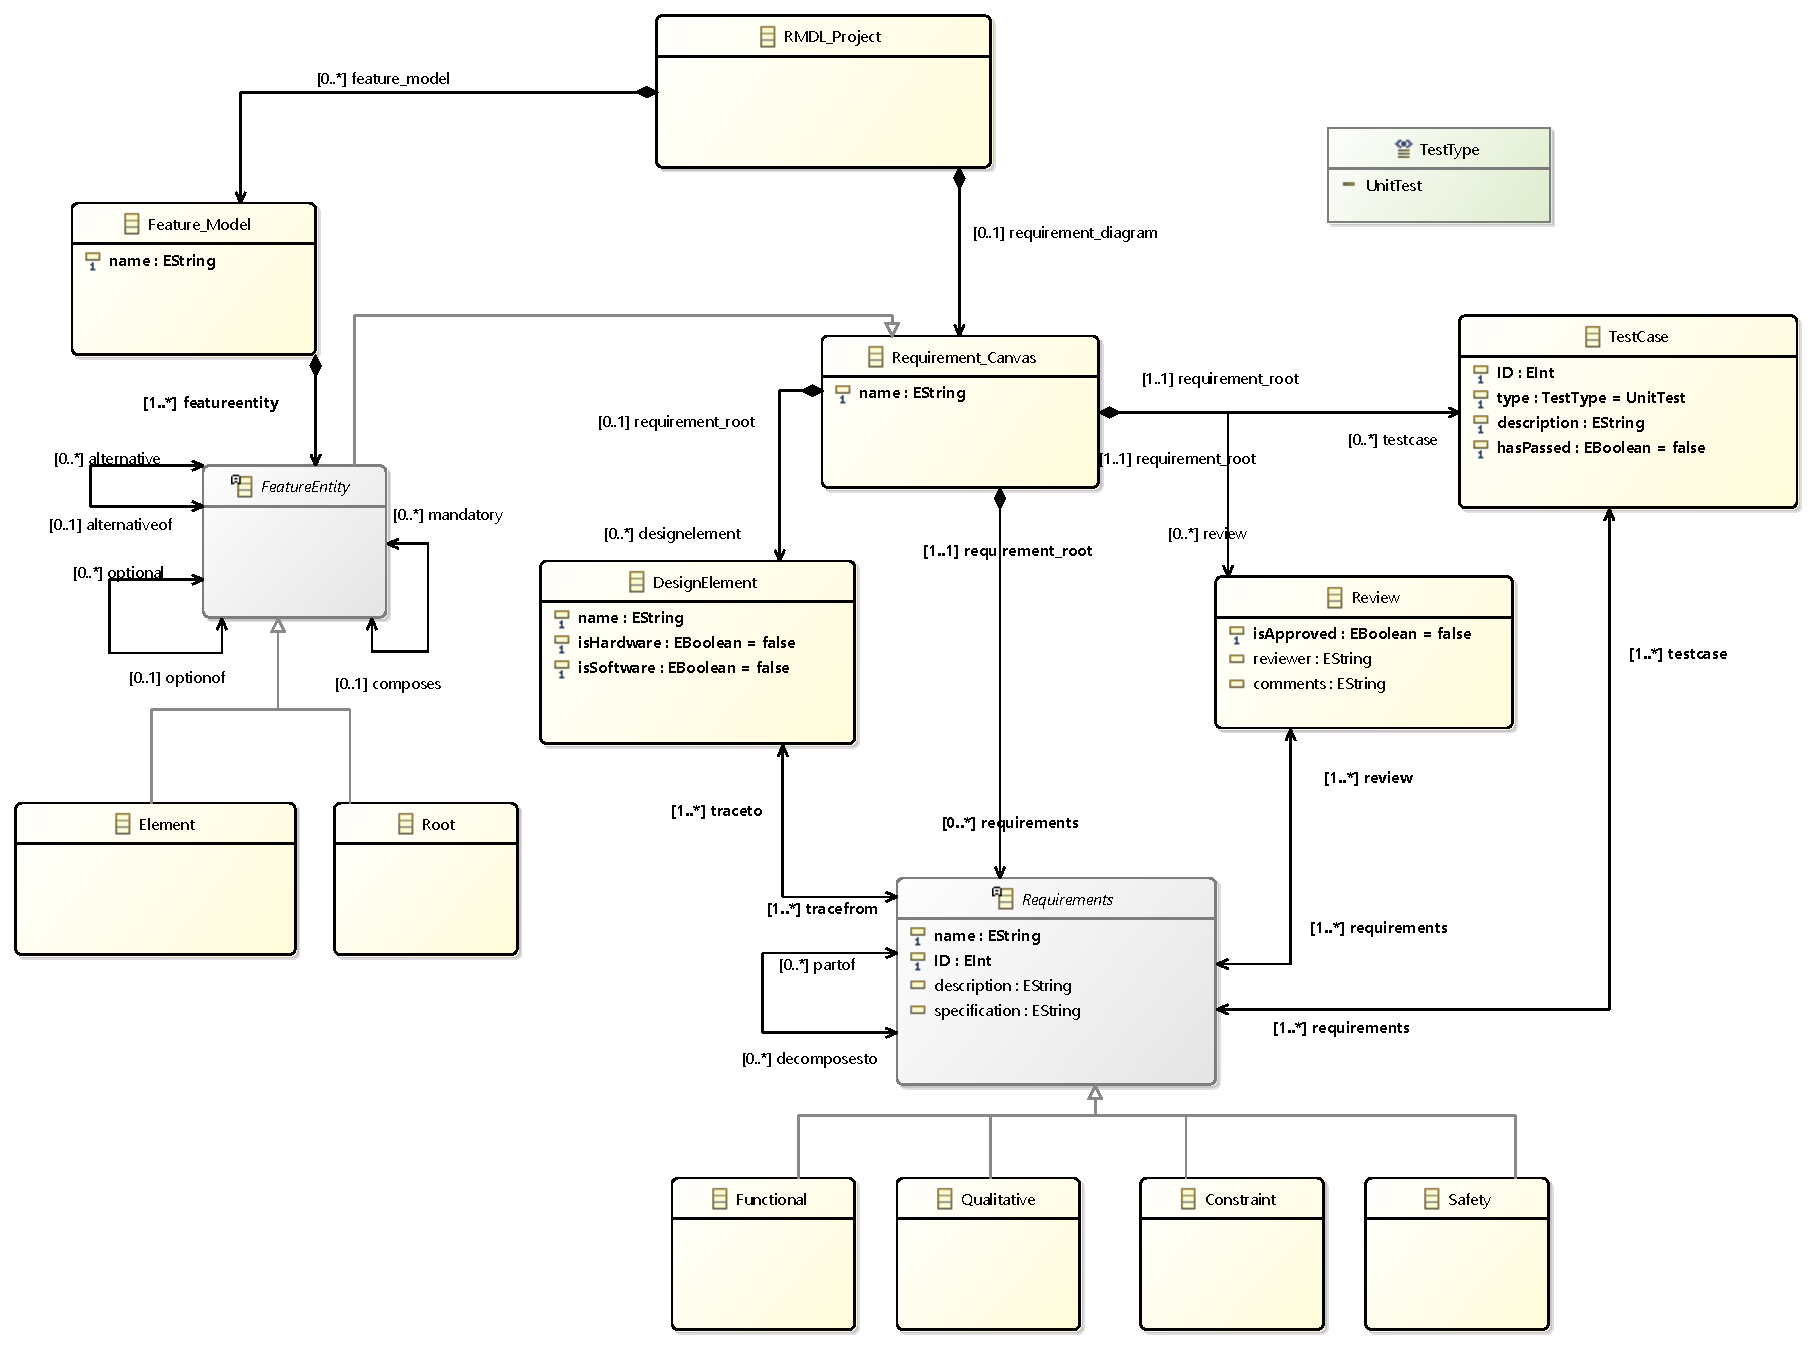
\includegraphics[width=\textwidth]{rmdl.pdf}
	\caption{CyclicL metamodel. Shows the specification for both the requirment canvas and feature modelling portions of CyclicL.}
	\label{fig:metamodel}
\end{figure}

We also added three more classes besides the requirements; \texttt{DesignElement}, \texttt{Review}, and \texttt{TestCase}. The test case and review classes are for verification and validation book-keeping respectively. This is also one of the reasons why we include design elements within the requirement canvas. The test cases are meant to determine if a requirement has been verified against its traced design elements while the review represents if the requirement has been validated. Currently, the verification and validation are expected to happen outside of \tool\ as it was out of scope for initial development. Design elements are also meant to be black boxes as we do not want to pollute our requirement environment with design aspects. We have limited it to determining if a design element is hardware, software, or neither (undetermined when building the requirements or an integrated system). Another reason for having design elements within the requirement canvas is to allow an opportunity for future development for design generation based on the requirements specified in \tool. We also have an enum \texttt{TestType}. This enum allows users to categorize the test users may want to apply to their requirements. At this time in development, only \texttt{UnitTest} is implemented as a type, but more can be added in future revisions.

For the feature modelling portion of the metamodel, the specification is based on the work of Peter H\"{o}fner et al.~\cite{hofner2006feature,hofner2011algebra} which uses set theory as the basis for proving how their feature modelling algebra works. It is also loosely inspired by FeatureIDE~\cite{kastner2009featureide, thum2014featureide} an extremely well-polished feature modelling plugin tool for Eclipse. The main reason we recreated the specification for feature modelling within \tool\ is to explore the implication of using features to encapsulate requirements. This is a key step in the process as this allows for what we dub feature-requirement traceability. As this proposed methodology suggests that features be used to encapsulate requirement to support feature-driven development efforts, having a way of representing that relationship in a formal specification such as a metamodel was impactful both for the development of \tool\ and the development of the concept.

\section{Feature-Requirement Traceability}

The feature-requirement traceability is the main purpose for this methodology. As previous steps have been taken to identify both the features and requirements of the system, this relationship between features and requirements is integral for the process. This relationship is captured by the inheritance connection between the \texttt{Requirement\_Canvas} and the \texttt{FeatureEntity} classes in the metamodel. By allowing every model element in the feature model to double as a requirement canvas, it allows each feature to contain all the model elements requirement for the requirement canvas thus encapsulating the various types of requirements, their associated approvals, and associated design elements.

This relationship allows for several key benefits. First, it allows for direct traceability between the requirements and their respective features. Since every requirement will be `owned' by a feature, we can easily trace the relationship between requirements within a feature, between various features, and within the entire system. Secondly, this modelling approach is more reflective of the relationship that features and requirement have in \ac{FDD} environments allowing more compliance between tolls that support \ac{FDD}. Thirdly, this allows us to model product variance at the requirement level. Allowing for specification of product variance is helpful for reducing unexpected changes and capturing knowledge of anticipated variance in product early in the product lifecycle development. Further, this will support change impact analysis across product variants to support product maintenance. 

Some anticipated downsides to this extension is that it might not be compatible with existing feature model composition approaches. Since every feature element now doubles as a requirement canvas this can break conventional feature composition strategies forcing us to create new ones. Another downside is handling requirements that can be related to multiple features. Due to the encapsulation strategy we are proposing, cross-cutting requirements across features is not supported at this time. There might be ways that users circumvent this which can lead to duplicated or inconsistent requirement across several features. 

\begin{figure}
	\centering
	\includesvg[width=\textwidth]{feature-requirement}
	\caption{Example of how a feature can be opened up to display encapsulated requirements.}
	\label{fig:feature-requirement}
\end{figure}

In figure \ref{fig:feature-requirement} we show the intention of having the features encapsulate the requirements. There is an explicit method for information hiding, and access to the requirements necessitates diving into a feature. This is where we transition from feature modelling to the requirement canvas. Within the canvas we can then define our requirements and specifications for the owning feature. 

\section{Requirement Specification}

Between the goal diagrams and use case diagrams we showed how we can do requirement refinement. In the requirement canvas we intend to express these requirements as well. This is beyond just refinement however, as part of the requirement canvas we also enable requirement specification. Currently we support behavioral specification through a loose implementation of Gherkin syntax~\cite{cucumberdocs}. The Gherkin style of specification is a structured natural language approach to specifying behaviors. It follows a pseudo predicate logic system using three main keywords; GIVEN, WHEN, and THEN. The GIVEN keyword is used to express behavioral preconditions. The WHEN keyword is used to express events that trigger some new behavior. These triggers can be either internal or external to the specified system. Finally, the THEN keyword is meant to specify behavioral postconditions. 

The reasons for using Gherkin style specifications in the requirement canvas is two-fold. We want to specification environment to be both easy to use and read. This provides a low barrier for entry to specify requirements and reading them. This increased flexibility is meant to both technical and non-technical people to specify system requirements. Secondly, while the flexibility is good, we still wanted some constraints for how specifications can be written. Rather than introducing some arbitrary constraints ourselves, Gherkin provided a nice off the shelf solution. Despite our current implementation not being completely faithful to the original specification, it is enough for a proof of concept.

\section{Requirement Based Feature Identification}

Due to the relationship between features and requirements outlined in this methodology there are alternative ways to identify features. The variation points that exist in this approach are the requirements held in the features. As a result, variant requirements can potentially identify new features previously missed by the \ac{UCD}. Thus far this methodology has been primarily top-down in the approach to identifying features using the domain analysis. However, it is expected that variant requirements will be identified during the elicitation process. This introduces the possibility for a bottom-up approach to identify features. Variant requirements elicited should still be supported by the goal diagram. Naturally, through this bottom-up portion of the methodology, it is encouraged to iterate on previous steps as engineers incrementally follow the approach.

\begin{figure}
	\centering
	\includesvg[width=\textwidth]{acc_fm}
	\caption{Simplified example of an adaptive cruise control feature model.}
	\label{fig:acc_fm}
\end{figure}

In figure~\ref{fig:acc_fm}, we can see a simplified feature model of an Adaptive Cruise Control (ACC) system. For the auto braking feature there are two alternative features available underneath denoted with the aggregation symbol at the source and open circle at the target. Sensor fusion requirements based on possible variant products (such as radar and camera versus lidar and sonar implementations) generate alternative features under the auto braking feature. Any requirements that can apply to both are expected to be abstracted up a feature to auto braking. This scoping is meant to reduce cross cutting concerns between features due to requirement dependencies.







	\chapter{Implementation}

As a proof of concept, we have implemented a \ac{DSL} to show the feasibility of automated traceability between features and requirements. Supported by the entire methodology, the tool \tool\ is a model-based tool to support to creation of feature models, requirement models, and leveraging the relationship between them to support automated traceability generation and maintenance throughout a products life-cycle.

\tool\ is also where we have been exploring potential composition strategies. We expected that traditional composition techniques from \ac{PLE} may require some modifications as a result of the relationship we have introduced between features and requirements. 

\section{Implementation Objectives}

\tool\ has a few objectives to satisfy as a proof of concept. We expect the main users of the tool to be engineers, primarily but not limited to software engineers. To be successful, \tool\ needs to allow users to create feature models so they can define their product families. \tool\ needs to have a way to define requirements. Since \tool\ is also an implementation of the methodology it also needs to use the relationship we have defined between features and requirements. Finally, since we want to support iterative and incremental development, \tool\ also needs to have some way to enhance the process of generating and maintaining traceability matrices for requirements and features. 

Based on our objectives, \tool\ has two main modelling environments that are distinct and connected. The first is the feature modelling half of the tool. The purpose of this modelling environment is to allow the user to define their product in terms of features. The second modelling environment is the requirement canvas environment. This environment enables the user to specify their requirements, associate requirements to design elements, and assign reviewers and test cases to requirements. This is also where the majority of the traceability in \tool\ is defined. These two modelling environments are connected through the features in the feature modelling portion. We use features to encapsulate the requirements. Each feature owns its requirements, allowing for a strong hierarchy between features and requirements. By connecting the two modelling environments we end up with a couple of different forms of traceability. Using the requirement canvases alone we can get a simple requirement traceability matrix. Using just the feature modelling environment we can generate feature traceability. And when we combine both environments we get a feature-requirement traceability matrix that shows what features own what requirements, and how they trace and relate to other requirements and features in the system. 

For the feature modelling portion of the tool, our specification is based on the same algebraic specification from Peter H\"{o}fner \textit{et al}~\cite{hofner2006feature,hofner2011algebra}, with a small extension to account for requirement encapsulation. We use this specification instead of making a new one to leverage previous proofs and work done on formal specifications for feature modelling. It saved us time and let us begin development much sooner. We consider the relationship between features and requirements within a product family as shown in figure~\ref{fig:spec}. By using this definition, we treat each feature as a set of requirements such that every requirement within the feature is unique. As stated in the definition however, it does not account for duplicate requirements in separate feature elements. This is something that will need to be handled in the implementation. This definition does allow us to scope and understand what we want a feature to do; namely encapsulate requirements.
\begin{figure}
\begin{align}
	\text{Let } \mathbb{F} \text{ be a set of arbitrary elements that we call features.}\\
		\text{We can call a collection (set) of features a product.}\\
		\text{The set of all possible products is } \mathbb{P} \overset{\mathrm{def}}{=} \mathcal{P}(\mathbb{F})\\
		\text{A collection of products (an element of } \mathcal{P}(\mathbb{P})\text{)}\\
		\text{is called a product line (or product family)}\\
		\text{This model does not capture feature duplication}\\
		\text{Let } \mathbb{R} \text{ be a set of arbitrary elements that we call requirements.}\\
		\text{We can call a collection (set) of requirements a feature.}\\
		\text{The set of all possible features is: } \mathbb{F} \overset{\mathrm{def}}{=} \mathcal{P}(\mathbb{R})\\
		\text{This model does not capture requirement duplication.}
\end{align}
\caption{Definition of the relationship between features and requirements.}
\label{fig:spec}
\end{figure}

%\begin{align}
%	\text{Let } \mathbb{F} \text{ be a set of arbitrary elements that we call features.}\\
%	\text{We can call a collection (set) of features a product.}\\
%	\text{The set of all possible products is } \mathbb{P} \overset{\mathrm{def}}{=} \mathcal{P}(\mathbb{F})\\
%	\text{A collection of products (an element of } \mathcal{P}(\mathbb{P})\text{)}\\
%	\text{is called a product line (or product family)}\\
%	\text{This model does not capture feature duplication}\\
%	+:\mathcal{P}(\mathbb{P}) \times \mathcal{P}(\mathbb{P}) \rightarrow \mathcal{P}(\mathbb{P})\\
%	P + Q = P \cup Q\\
%	\therefore \mathcal{P}(\mathbb{P}) \times \mathcal{P}(\mathbb{P}) \rightarrow \mathcal{P}(\mathbb{P})\\
%	P \cdot Q = \{p \cup q : p \in P, q \in Q\}\\ 
%	1 = \{\emptyset\} \text{ denotes the product line consisting}\\
%	\text{ of the empty product that has no features}\\
%	\emptyset \text{ is the zero}\\
%	\text{The structure:}\\
%	\mathbb{P}FS \overset{\mathrm{def}}{=} (\mathcal{P}(\mathbb{P}), +, \emptyset, \cdot, \{\emptyset\})\\
%	\text{forms a product line algebra}\\
%	\text{Let } \mathbb{R} \text{ be a set of arbitrary elements that we call}\\
%	\text{requirements.}\\
%	\text{We can call a collection (set) of requirements a feature.}\\
%	\text{The set of all possible features is: } \mathbb{F} \overset{\mathrm{def}}{=} \mathcal{P}(\mathbb{R})\\
%	\text{This model does not capture requirement duplication.}
%\end{align}

\begin{figure}[hbt!]
	\centering
	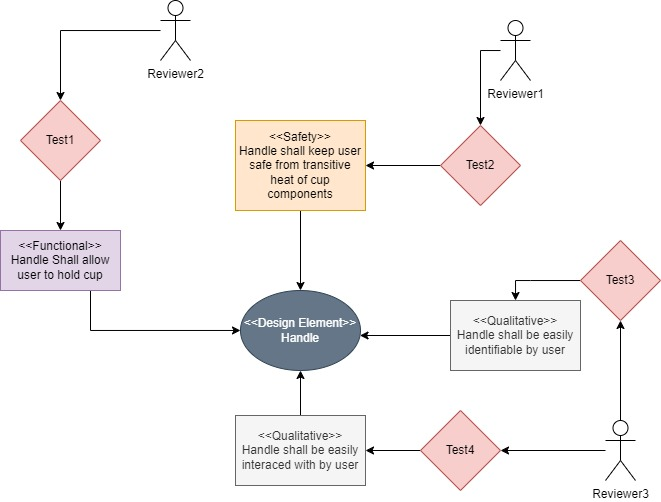
\includegraphics[width=\columnwidth]{Figures/CoffeCup_ReqModel.jpg}
	\caption{Example of a requirement canvas concrete syntax. The example uses a disposable coffee cup with a handle as the focus of the diagram.}
	\label{fig:CoffeCup_ReqModel}
\end{figure}

Our main reason for using requirement diagrams as a starting point to capture requirements is the semi-formal specification in SysML for requirement diagrams. We found enough semantics in the specification to enable traceability automation using the connections between elements. Furthermore, requirement diagrams are a generally under-explored means of requirement engineering based on our literature review, especially when compared to feature modelling and product line engineering. This led to us deciding to iterate on requirement diagrams as a means of exploration for traceability, supporting our previous decision to reuse as much as possible from previous \ac{PLE} work. In this exploration, we diverged significantly from the original specification for requirement diagrams. In order to capture this divergence, we henceforth refer to the requirement modelling environment as the requirement canvas. We will explore more of the differences in sections \ref{sec:Abstract_Syntax} and \ref{sec:Concrete_Syntax}.

An existing tool for PLE and feature modelling such as FeatureIDE~\cite{kastner2009featureide, thum2014featureide} allows for product generation by weaving software defined in the features together. GEARS~\cite{GEARS} has a three-tiered approach to PLE that can help with software management. However, neither of those tools has an explicit focus on traceability between features and requirements. The requirements are housed separately from the feature model and necessitate user intervention to pull requirements from another source, if at all since the tools can function fine without requirements. However, in \tool\ the requirements are necessary to build out the full traceability that the tool is focused on generating and maintaining, functionality that is lacking or not the primary focus in other PLE tools. Thus, we position \tool\ as a development tool that automates traceability generation and maintenance between PLE and requirement engineering by purpose-building it for feature model and requirement canvas creation. By housing everything in one location it prevents a situation where the feature model and requirements can be out of sync with each other. We propose that having both within a single tool facilitates auxiliary development activities such as change impact analysis and automated maintenance of traceability documentation.

\subsection{Goals and Limitations}

In figure~\ref{fig:CyclicL_goals} we capture some anticipated goals for our end-users. In conjunction with our own objectives we use these to support our high-level requirements for \tool. As the scope of the tool is currently only focused on the traceability portion of the methodology we have scoped user goals to be after they have completed an independent domain analysis. We assume that users have their supporting documentation when using \tool. This is a limitation of the tool for now as we do not currently support traceability from the domain analysis to the identified features and requirements. We also have no way to encourage or enforce a domain analysis purely through the use of \tool. Thus, we cannot confirm validity of models created in \tool\ at this time based on justifications from supporting documentation.

\begin{figure}
	\centering
	\includesvg[width=\textwidth]{CyclicL_goals}
	\caption{Anticipated goals of users for \tool.}
	\label{fig:CyclicL_goals}
\end{figure}

\subsection{Requirements}
We extracted high-level requirements from the previous work in building a product line and requirements for a coffee cup to guide initial development plans for \tool~\cite{chiang2024mapping}. We also included the goal of supporting iterative and incremental development life-cycles. We define an iterative change as a change based on feedback from later stages of development or stakeholders. These are usually larger changes relative to an incremental change. Examples of an iterative change can include a new version of a development artifact or a redesign of a development artifact. Incremental changes are changes that are usually smaller in scope, and bound within a single development phase. Examples of an incremental change can be a refactoring change, updating a definition, or changing a connection between components. Our initial list of requirements was as follows:

\begin{itemize}
	\item Tool shall provide the user with an environment for defining requirements.
	\item Tool shall provide the user with an environment for defining features.
	\item Tool shall allow the user to specify design elements.
	\item Tool shall allow the user to relate one or more requirements to one or more design elements.
	\item Tool shall allow the user to use features to capture and own requirements.
	\item Tool shall automatically create and maintain a traceability matrix.
	\item Tool shall facilitate iterative development of the requirements canvases (\textit{note:} this remains as ongoing work).
	\item Tool shall facilitate incremental development of the requirements canvases.
\end{itemize}

Under these specifications, we allow for requirement encapsulation. We treat the requirements encapsulated by a feature as attributes and are considered feature requirements, thus scoped by the feature. For the structure to define the requirements within a feature, we decided to use requirement diagrams from the SysML specification~\cite{sysml2019omg} as inspiration for creating our requirement canvas. For a rough idea of what we wanted the requirement canvases to look like we sketched requirements for a disposable coffee cup with a handle, shown in Figure \ref{fig:CoffeCup_ReqModel}.


\section{Abstract Syntax}
\label{sec:Abstract_Syntax}

The metamodel shown in figure~\ref{fig:metamodel} is what was used for building \tool. The abstract syntax can be roughly divided into two main portions; the feature model and the requirement canvas, mirroring our requirement decisions for \tool. The requirement canvas portion of the metamodel is not a complete implementation of the SysML specification for requirement diagrams. We decided to implement enough to allow us to model requirements sufficiently to get traceability. To enable features to encapsulate requirements, the \texttt{FeatureEntity} class inherits from the \texttt{Requirement\_Canvas} class. Thus, every feature in the feature model can become a requirement canvas, allowing us to capture the requirements for each feature as attributes of said feature. There are three defined relationships for features; mandatory, alternative, and optional. These are specified with bidirectional references to allow visibility in either direction from any feature. This decision was made to enhance the traceability available in the modelling environment and simplify development for the traceability matrices. The multiplicities are also defined with 0..1 at the top end to limit how the feature composition will work. This limits how many nodes a leaf element can be connected to, constraining what models can be built and simplifying the feature composition. The requirement canvas also has a containment relationship with the model root, \texttt{RMDL\_Project}. This is carried over from earlier development and was left in the tool, for now, to allow users to define a requirement canvas for the entire system they are specifying without being tied to specific features. The justification for this structure is to provide a kind of doodle space for requirement specification that can later be refined by copying and pasting some model elements into a requirement canvas encapsulated by a feature. However, to prevent cluttering instantiated projects with too many disconnected drawing spaces we limit the multiplicity to [0..1].

Next, for the requirements in the requirement canvas, we identified four requirement categories; \texttt{Functional}, \texttt{Qualitative}, \texttt{Constraint}, and \texttt{Safety}. Functional requirements follow their traditional definition; things that a product or system must do. Qualitative requirements are identified as requirements that affect the way a product or system accomplishes its function. These include the look, feel, usability, humanity, and some performance requirements that are not categorized as functional. Constraint requirements are identified as requirements that add limitations of some type to a product or system. These include operational, environmental, maintainability, support, security, cultural, political, and legal requirements. These requirement definitions can be found in James and Suzanne Robertson Volere requirements~\cite{robertson2000volere}. Finally, safety requirements are critical as they identify all requirements that have to do with the safety of users or stakeholders involved in the function of a product or system. We highlight safety requirements as a separate requirement category as our target domain for \tool\ is safety-critical development. It is important to note that requirement categorization relies heavily upon system, or in \tool, feature scoping. For a safety feature, a safety requirement may be considered a functional requirement due to the feature scope. A functional feature, however, may contain safety requirements that are distinctly different from the functional requirements. This distinction relies heavily upon the capabilities of the engineer creating the models.

We also added three more classes besides the requirements; \texttt{DesignElement}, \texttt{Review}, and \texttt{TestCase}. The test case and review classes are for verification and validation book-keeping respectively. This is also one of the reasons why we include design elements within the requirement canvas. The test cases are meant to determine if a requirement has been verified against its traced design elements while the review represents if the requirement has been validated. Currently, the verification and validation are expected to happen outside of \tool\ as it was out of scope for initial development. Design elements are also meant to be black boxes as we do not want to pollute our requirement environment with design aspects. We have limited it to determining if a design element is hardware, software, or neither (undetermined when building the requirements or an integrated system). Another reason for having design elements within the requirement canvas is to allow an opportunity for future development for design generation based on the requirements specified in \tool. We also have an enum \texttt{TestType}. This enum allows users to categorize the test users may want to apply to their requirements. At this time in development, only \texttt{UnitTest} is implemented as a type, but more can be added in future revisions.

\section{Concrete Syntax}
\label{sec:Concrete_Syntax}

The design decisions towards the development of the concrete syntax for the requirement canvas follows the ideas from the Physics of Notation~\cite{5353439}. Various colors and shapes were used to maintain a bijective relationship between the concrete syntax and intended semantics. For example, in figure~\ref{fig:concrete_syntax_req_diag} all of the requirements have the same shape to show they have commonality as they inherit from the \texttt{Requirement} type, but use different colors to differentiate themselves from each other. Similarly, \texttt{Test Cases} and \texttt{Reviews} are dynamically colored to show when they pass/fail and approved/unapproved respectively. Finally, the \texttt{Design Element} symbols dynamically change color if they are stereotyped as software, hardware, or black-boxed.

\begin{figure*}[hbt!]
	\centering
	
\includegraphics[scale=0.043]{Figures/Requirement Diagram_SteeringWheel.jpg}
	\caption{An example of the concrete syntax for the requirement canvas using requirements from the automotive domain.}
	\label{fig:concrete_syntax_req_diag}
\end{figure*}

For the feature modelling portion of \tool, we maintained as close to traditional syntax as possible. This is due to the objective of maintaining the original specification for feature modelling to our best ability during implementation. Given some of the default limitations of Sirius there are still some differences. 

Figure~\ref{fig:concrete_syntax_feat_mod} shows an example product family created in \tool. The root of the model is shown in the grey box and the features of the model use white circles. The mandatory reference uses the black diamond at the source and an arrow at the target. The optional relationship uses no decorator at the source and a triangle at the target. This is to represent OR relationships. The alternative reference uses a white diamond at the source and a triangle at the target. This is to represent XOR relationships. As this is a top-down modelling layout, the reference source is towards the top and the reference target is towards the bottom. The optional and alternative references share the diamond at the target to show that the target is optional. In contrast, the white diamond at the source differentiates the two types of references. Thus while they have some common semantics in the options, the alternative has more syntax to represent its extended semantics.

\begin{figure}[hbt!]
	\centering
	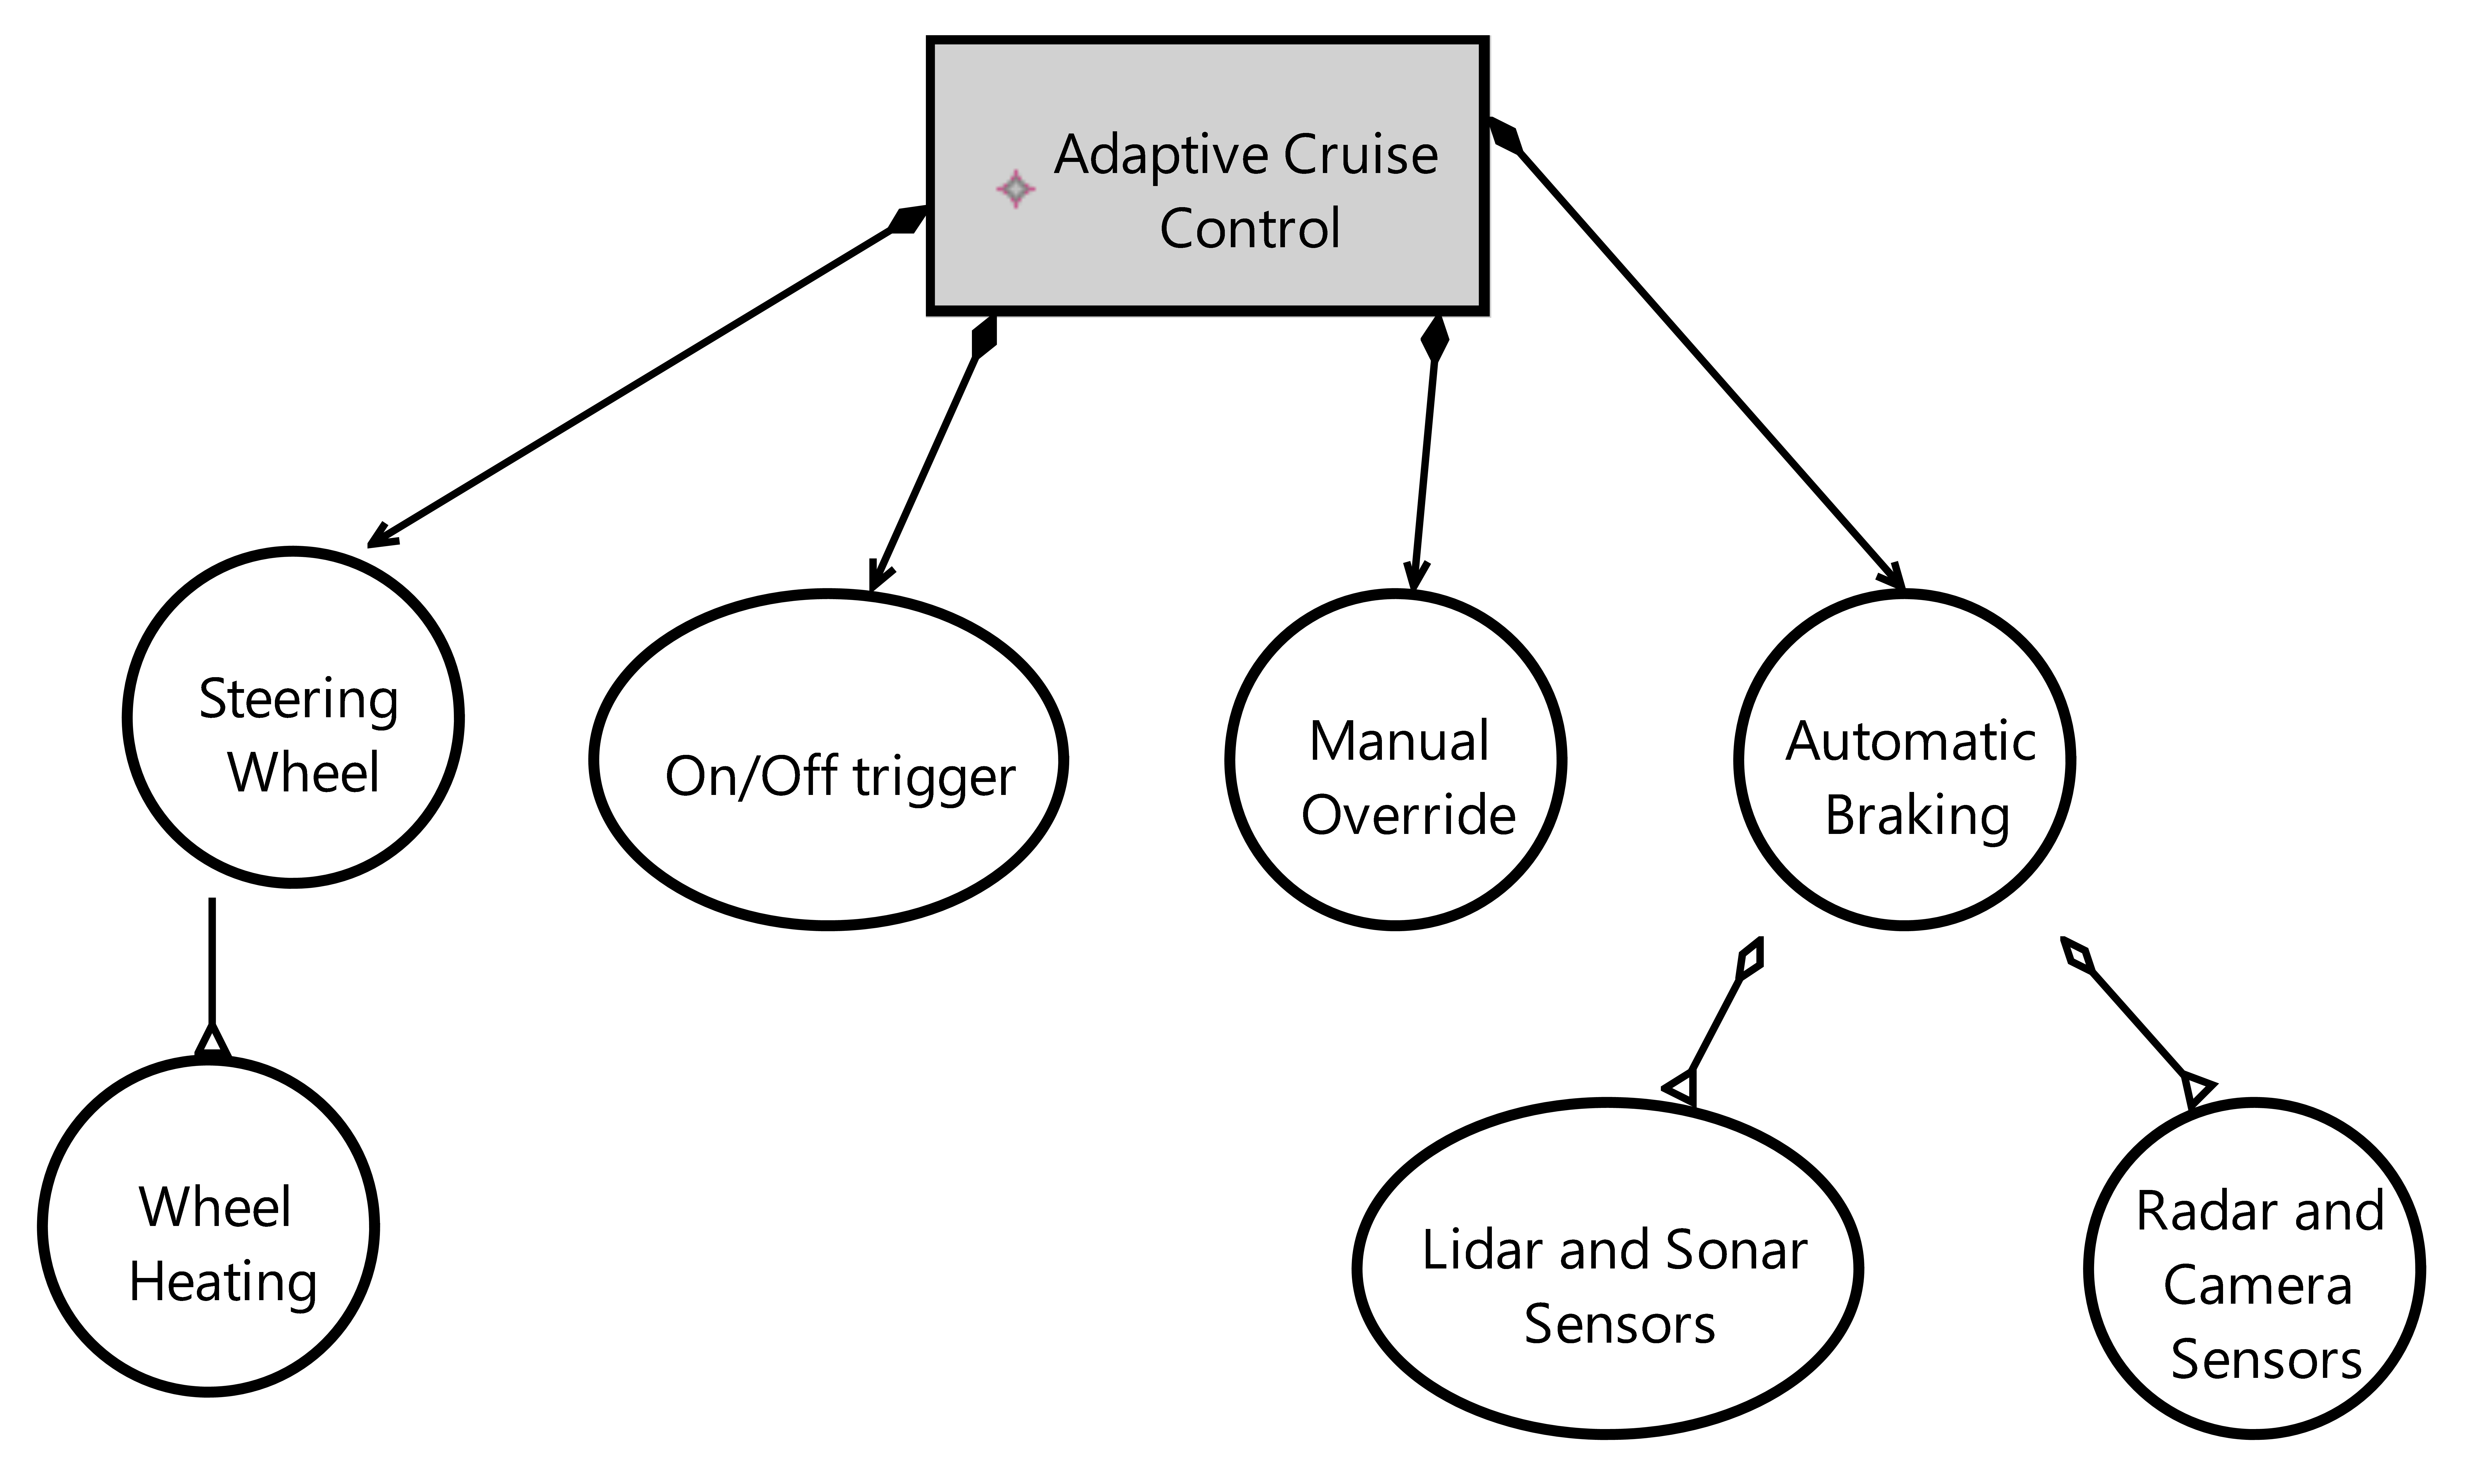
\includegraphics[width=\columnwidth]{Figures/FeatureModel_acc.jpg}
	\caption{An example of the concrete syntax for the feature model using features for an adaptive cruise control system from the automotive domain.}
	\label{fig:concrete_syntax_feat_mod}
\end{figure}

Along with the graphical portion of \tool, we also implemented an Xtext-based~\cite{eysholdt2010xtext} specification language. The implemented specification language is based on the Gherkin specification language~\cite{nicieja2017writing, cucumberdocs}. We chose this as the specification language for our requirements for a few reasons. Gherkin uses a structured natural language for specifications, thus making it relatively approachable for users when defining their requirements. Further, despite using natural language, it uses keywords to provide a predicate logic structure to the specifications. The keyword `Given' is used for preconditions, `When' is used for events, and `Then' is used for postconditions. The combined approach of adding predicate structure to natural language makes it relatively easy to specify requirements and to implement the language within \tool. 

\begin{figure}
	\begin{lstlisting}
		Given{
			Precond FeatureExists: "Steering wheel has heating feature."
			Precond CarIsOn: "Vehicle is on."
		}
		When{
			Event UserTurnsOnHeating: "User interacts with heating interface to turn on/off wheel heating."
		}
		Then{
			Postcond StateChange: "Wheel heating boolean changes state to on or off depending on current state."
		}
	\end{lstlisting}
	\caption{Gherkin specification for Wheel Heating on/off functional requirement. The high-level requirement description is: User shall be able to turn wheel heating on/off.}
	\label{fig:specification}
\end{figure}

\section{Design Decisions}

A major design decision for \tool\ was using our own implementation for feature modelling. Other tools such as FeatureIDE already exist and are native to Eclipse. We decided to use our own implementation to remove possible constraints of having to work with an existing tool so that we can focus on the traceability aspects of the tool. Another reason was to allow us some flexibility in how to implement the compositional relationship between features and requirements. As we were not sure how best to implement the relationship to support. Further, this gave us flexibility to explore how we might want to navigate the created models and traceability matrices. 






\subsection{Composition Implementations}

The relationship between features and requirements makes traditional composition techniques for \ac{PLE} a challenge. Given the convention that a requirements variant necessitates a new feature, composing features and requirements to a product is relatively straightforward at this time. Currently, the approach focuses on the features themselves for the composition, with the assumption that each feature has unique requirements. If a requirement applies to multiple features then it is meant to be abstracted up a level in the tree to a higher feature. This currently reduces cross cutting concerns and dependencies between requirements. This allows users to define the necessary constraints and rules for how the features within a model are allowed to compose to a product (every car needs 4 wheels for example). As of the time of writing more complex analysis is planned for future work, however for a proof of concept this is currently feasible in \tool.


	\chapter{Evaluation}

Throughout this thesis we have been using the automotive domain to tell the story of how to use this methodology and \tool. This is because within the automotive domain we can find two of the main issues we are addressing with this proposal; how to handle variants within a product family and maintaining traceability throughout the product stacks. For automotive manufacturers there are variants in the customer facing product, evident in the different vehicles that are offered, the different model years between vehicles, and the various trims that are available within a single vehicle model. There are also variants that can exist internal to the manufacturer as they go through development and decompose the vehicle into it's components; engine, transmission, cooling, heating variants that are used across platforms for example. Managing these portfolios, across multiple levels of abstraction necessitates product family traceability in order to keep track of requirements constraints that lead to the various design and implementation decisions. 

For the evaluation portion of this thesis, we look towards the medical domain and medical device development. There is a lot of overlap between medical device development and automotive manufacturing. The medical device we will be using for this evaluation is a pacemaker. From the perspective of safety criticality, medical devices such as a pacemaker tend to have a greater impact on individual health and safety which is often reflected in medical regulations. Regional legislation may affect product development and the products themselves may have variants based on the capabilities of target stakeholders, in this case individual patients. For this thesis we keep in mind medical device guidelines and classifications based on Health Canada regulations~\cite{CanadaGuidanceDocument, VerifyDevices} as we are from a Canadian institution. This means that a pacemaker would be a class 4 medical device.

This evaluation will use an existing requirement document from Boston Scientific~\ref{apdx:Req} for pacemaker development. The pacemaker requirement document we have chosen is often used as part of the undergraduate curriculum at McMaster University for teaching product life-cycle development and safety-critical development. We will be assessing how this methodology and tool can be used to improve an existing requirement set, create traceability between features and requirement, and potential integration points with a development process. 

%Specifically, we are looking at a requirement set from Boston Scientific for a pacemaker~\ref{apdx:Req}. This requirement set is often used as part of the undergraduate curriculum at McMaster University for teaching product life-cycle development and safety-critical development.

%From the perspective of safety criticality, medical devices and a pacemaker especially, tend to have a greater impact on individual health and safety. Regional legislation may affect product development and the products themselves may have variants based on the capabilities of target stakeholders, in this case individual patients. For this thesis we focus on medical device guidelines and classifications based on Health Canada legislation~\cite{CanadaGuidanceDocument}. 

\section{Knowledge Capture \& Domain Analysis}

%Method works for automotive requirements. Will show using pacemaker. Do not show generality. Just show that it works in two domains. Would be interesting to explore generality. 
%
%\begin{itemize}
%	\item Want to show benefit of methodology for capturing knowledge prior to requirement elicitation process. Benefit around requirement justification, communication, and stakeholder confirmation (last two are difficult to show, but easy to claim). Future work for proving this claim. Maybe make assurance case for this claim?
%	\item Want to show uncertainty and incompleteness management/control/mitigation of requirements using the scenario breakdowns of the requirement refinements. Might want to argue more about potential to better manage incompleteness and uncertainty. Can provide clarity on requirements, requirement refinement, and requirement decomposition. Evaluates characteristic of methodology rather than empirical property.
%	\item Want to show cost savings of modelling requirements compared to in other tools when it comes to requirement traceability
%	\item Want to show benefits of using product family to contain requirements.
%	\item Want to show benefits of tying development strategies of FDD with product family.
%	\item Want to show how scenario breakdown for refinement helps with specification using Gherkin.
%\end{itemize}

The first step in this proposal is examining how the domain analysis is conducted. This part of the evaluation examines how we can enhance existing knowledge capture approaches by introducing domain analysis techniques introduced in our methodology. Using the proposed processes, along with \tool, we will be assessing for the ability to find gaps in the original pacemaker requirement document, potential integration points for existing development process, and general enhancements for engineering practices.

%\ac{MDE} concepts to support later stages of development, including traceability and iteration.

\subsection{Goal Diagrams}

The full requirement set by Boston Scientific for a pacemaker is available in the Appendix~\ref{apdx:Req}. Though not explicitly stated as domain analysis, there is some knowledge capture that occurs in chapters 1 and 2 of the pacemaker requirements all captured in natural language. In fact, all the requirements specified by Boston Scientific are captured in natural language. These two chapters introduce the scope of the requirements, identify some of the stakeholders, and define the system and sub-systems. We found it sufficient for the engineers to have an idea of why the system is needed, who they are building it for, where its intended usage environment is, and why it is needed. We now attempt to improve this domain analysis using the goal diagram and  \ac{UCD} approaches outlined in our proposed methodology.

%do a good job of introducing the scope of the requirements, stakeholder identification, and system definitions. Enough for the engineers to have an idea of why the system is needed, who they are building it for, where its intended usage environment is, and why it is needed. We have found however that we can improve upon this domain analysis with the usage of goal diagrams and use case diagrams introduced by our proposed methodology.

\begin{figure}
	\centering
	\includesvg[width=\textwidth]{Pacemaker_lifecycle}
	\caption{Pacemaker lifecycle as outlined by Boston Scientific requirements.}
	\label{fig:Pacemaker_lifecycle}
\end{figure}

We follow the same pacemaker lifecycle outlined the requirement document shown in figure~\ref{fig:Pacemaker_lifecycle}. The lifecycle provides context for what the goals of our stakeholders would be throughout the life of the pacemaker. We find that the document explains what is necessary from the pacemaker during each stage of its lifecycle. The document does not however explain what each stage actually is. The stakeholder roles, use cases, or goals are also not defined our outlined for each stage throughout the product lifecycle. This can reduce the engineers' understanding of the product, and impact confidence in the requirements specified for product development.

The lack of context and knowledge can become a source of uncertainty during development. The extra definitions or knowledge of the stakeholder goals may not always result in a direct impact on the product features or requirements, however the ability to draw this conclusion from a body of knowledge is important to increase confidence in creating more complete and correct sets of features and requirements. To accomplish part of this domain analysis we performed a casual interview with a doctor to provide some perspective and insight to what some stakeholder goals might be outside of the perspective of the engineer responsible for development. Ultimately, this was a benefit as the doctor helped to provide some context missing from the original pacemaker specification.

%While perhaps not directly relevant to the requirements of the pacemaker, the lack of context can become a source of uncertainty during development. As such, the engineer may not know what information might be missing and therefore could become uncertain if the missing information is relevant to the requirements. As part of this domain analysis we performed a casual interview with a doctor to provide some perspective and insight to what some stakeholder goals might be outside of the perspective of the engineer responsible for development.


%capture provides uncertainty. As such, the engineer doe not know what information might be missing and therefore would not know if the missing information is relevant to the requirements. As part of this domain analysis we performed a casual interview with a doctor to provide some perspective and insight to what some stakeholder goals might be outside of the perspective of the engineer responsible for development.

The first step we took in this domain analysis is to provide some more information around what happens in each stage of the pacemaker lifecycle.

\begin{enumerate}
	\item \textbf{Pre-Implant:} This stage is where the patient is assessed if a pacemaker is required for their benefit. This stage includes risk/benefit discussion, patient risk tolerance, and informed patient consent. The patient has right to refuse care and may deny getting a pacemaker altogether. 
	\item \textbf{Implant:} This stage is the surgery. Straightforward stage, the patient undergoes surgery to implant the pacemaker.
	\item \textbf{Follow-up:} This stage occurs directly after the pacemaker is implanted. The patient is assessed for surgery safety (correct implantation of the pacemaker, no infection, no other surgical complications etc).
	\item \textbf{Ambulatory:} This stage is the regular day-to-day life of the patient post-surgery. This include regular check-ups with the patient's medical team. Regular assessment of the pacemaker is performed at this stage. If necessary, pacemaker maintenance or updates may be required. In extreme or unusual cases, pacemaker removal may be required or refused.
	\item \textbf{Explant:} This stage is where a pacemaker is removed from the patient. Extremely unlikely to be assessed as needed and even less likely to occur during the patients lifetime. However the pacemaker may still be removed after patients death.
	\item \textbf{Disposal:} This stage is when a pacemaker has reached end of life and is safely disposed.
\end{enumerate}

These definitions are helpful to engineers to get a better understanding of the complete product lifecycle after development. It helps to inform some of the goals that the various stakeholders may have, providing some insight into why the requirements are specified as such. Further, these extra definitions also helped us to identify more stakholders of the system beyond the original specification. The new list of stakeholders is the following:

\begin{itemize}
	\item Patient (from Pacemaker requirements)
	\item Patient Family
	\item Doctor (from Pacemaker requirements)
	\item Hospital
	\item Nurse (from Pacemaker requirements)
	\item Technician (from Pacemaker requirements)
\end{itemize}

The patient family was identified as another stakeholder of the pacemaker system due to some of the goals that were identified for both the patient and doctor stakeholders. One of the goals for doctors is to help the patient family navigate the health care system. Which informed us that the patients family are also stakeholders of the pacemaker system as they are likely to be involved with the patient quality of life. This ties into another goal we identified for the patient which is to regain or maintain a desired quality of life. The goals of the doctor and the patient stakeholders can be found in figures~\ref{fig:doctor_goals} and~\ref{fig:patient_goals} respectively.

\begin{figure}
	\centering
	\includesvg[width=\textwidth]{doctor_goals}
	\caption{Doctor goals in the context of the pacemaker system.}
	\label{fig:doctor_goals}
\end{figure}

One important belief that is important to identify is the patient belief \texttt{We all die eventually}. This leads to the patient goal of right to refuse care. This is critical to recognize patient autonomy in general. In the specific case around the pacemaker it presents itself twice; a patient can refuse to implant the pacemaker and can refuse to explant the pacemaker. Refusal to implant the pacemaker is less common, but informed consent is an important part of the process before a doctor can implant the pacemaker. More commonly, especially with pacemaker failure, the patient can refuse to have the pacemaker explanted. This can be for a multitude of reasons, but often it is simply because the patient is old and does not want surgery. We point this out as a gap in the original specification as this can have requirement and design implications.

\begin{figure}
	\centering
	\includesvg[width=\textwidth]{patient_goals}
	\caption{Patient goals in the context of the pacemaker system.}
	\label{fig:patient_goals}
\end{figure}

We also identify what the goals are for the nurse and technician stakeholders. This helps to clarify what roles they would play in the context of the pacemaker lifecycle. During the ambulatory stage, the patient will be spending a lot of time with the nurse to monitor health and functionality of the pacemaker. The technician may be called if there is a bug detected for troubleshooting, and in the extreme cases, disposal of the pacemaker. We also add what the goals of the hospital could be, though the hospital is mostly where the resources are sourced. There can be more goals for the hospital in general, but for this context we limited the goals to the scope of a patient with bradycardia and the pacemaker lifecycle.

\begin{figure}
	\centering
	\includesvg[scale=0.7]{hospital_goals}
	\caption{Hospital goals in the context of the pacemaker system.}
	\label{fig:hospital_goals}
\end{figure}

\begin{figure}
	\centering
	\includesvg[scale=0.6]{nurse_goals}
	\caption{Nurse goals in the context of the pacemaker system.}
	\label{fig:nurse_goals}
\end{figure}

\begin{figure}
	\centering
	\includesvg[scale=0.7]{patient_family_goals}
	\caption{Patient family goals in the context of the pacemaker system.}
	\label{fig:patient_family_goals}
\end{figure}

Along with the hospital, we identified another stakeholder beyond the scope of the original pacemaker requirement; patient family. The reason we include the patient family as a stakeholder is because they are also relevant to the pacemaker lifecycle as a potential resource for the patient. The patient family also will likely share the goal to help care for the patient, performed in ways that the medical team is unable to; help in the day-to-day activities of the patient and in the community.

\begin{figure}
	\centering
	\includesvg[scale=0.7]{technician_goals}
	\caption{Technician goals in the context of the pacemaker system.}
	\label{fig:technician_goals}
\end{figure}

\begin{figure}
	\centering
	\includesvg[width=\textwidth]{nurse_doctor_combined}
	\caption{Combined nurse and doctor goals.}
	\label{fig:nurse_doctor_combined}
\end{figure}

There are many goals we identified that are shared across stakeholders. We have them as separate bubbles for the sake of displaying in this thesis, but another potential benefit of the goal diagrams is that we can create venn diagrams that explicitly show the overlap between stakeholders and reduce copied goals. We show the combined goals of the doctor and nurse stakeholders in figure~\ref{fig:nurse_doctor_combined}.

Thus far with the goal diagrams we have identified two more stakeholders that were not identified in the original requirement document. We have provided insight into what some of the goals are for each of the stakeholders, along with supporting beliefs, tasks, and resources. We can claim that we have reduced some uncertainty around what goals the stakeholders would have in regards to the pacemaker product lifecycle. We also claim that we have provided some extra context around the stages of the pacemaker lifecycle that can help inform or support decisions for the requirements and subsequent development.

\subsection{Use Case Diagrams}

The next step we want to take is identify the use cases for each of these stakeholders, if they have uses, and compare them with the identified uses of the original requirement document. Many of the tasks (from the goal diagrams) that we have identified for the stakeholders do not require the pacemaker system to complete, but the goals do. According to the proposed methodology, we want to identify the use cases that the stakeholders will need the pacemaker system for. These use cases should also be traceable to one or more goals for the stakeholders. This traceability is important to justify the identified use cases.

In chapter 2: System Definition for the pacemaker requirements document it defines the various components that compose the pacemaker system; the pacemaker device (also known as the pulse generator or PG), the Device Controller-Monitor and associated software, and the device leads that are implanted in the patient. Those three components become the boundaries of our UCDs. This is an easy integration point between out methodology and the existing documentation. We can save some time by reusing the system and sub-system decompositions from the original document. The document does not explicitly state what the features or use cases are for each of the devices, but there are overview sections that we can use as a starting point for determining what the use cases are.

The PG device overview provides the following information:
\begin{itemize}
	\item Monitor and regulate patient heart rate.
	\item Detect and provide therapy for bradycardia conditions.
	\item Provide programmable, single- and dual-chamber, rate-adaptive pacing, both permanent and temporary.
	\item In adaptive rate modes, an accelerometer is used to measure the physical activity resulting in a sensor indicated rate for pacing the heart.
	\item Programming and interrogation via bi-directional telemetry from the DCM. Allows physician to change operating mode of parameters of the device non-invasively after implantation.
	\item Provide the following historical data:
	\begin{itemize}
		\item Sensor output data.
		\item Atrial and ventricular rate histograms.
	\end{itemize}
	\item In conjunction with DCM, provide diagnostic features including:
	\begin{itemize}
		\item Real time telemetry markers
		\item EGMs
		\item P and R wave measurements
		\item Lead impedance
		\item Battery status tests
	\end{itemize}
\end{itemize}

The overview for the DCM contains two sub-systems; a hardware platform and pacemaker application software. It also outlines the role of the DCM. The DCM is the primary implant, pre-discharge EP support, and follow-up device for the pacemaker system. It is capable of being used in the operating room, the doctor's office and the eletrophysiology lab. The DCM communicates with the PG using its software and hardware sub-systems. The DCM overview provides the following information:
\begin{itemize}
	\item Program and interrogate a pacemaker.
	\item Command delivery of ``Pace-Now" pace.
	\item Acquire and show diagnostics (history) and lead signal measurement information.
	\item Acquire and show sensor history and trending information.
	\item Show visible and audible indications of communication between the DCM and PG device, including beeping and LED's for alerting the operator to error conditions.
	\item Acquire and show multi-channel monitoring including surface electrogardiogram and telemetered signals (e.g. EGM, annotated event markers).
	\item Print reports and strip charts.
	\item Monitor battery status.
	\item Output to external strip chart recorders.
	\item Manage windows for display of text and graphics.
	\item Set the date and time.
\end{itemize}

The lead system overview provides the following information:
\begin{itemize}
	\item The lead system implanted in the patient allows the device to sense intrinsic activity of the heart's electrical signals and delivers pacing therapy to the patient's heart.
	\item The leads are connected to the PG via its header. All IS-1 bipolar leads are supported.
\end{itemize}

Taking into account the various overviews we can begin to create the UCDs. A helpful insight that the overviews provide that has been missed thus far is the way the sub-systems will interact with each other. In the scope of the UCDs, we can model this by treating the various sub-systems as stakeholders in the diagram environment. Interpreting the overview for the PG device we can have the UCD shown in figure~\ref{fig:pg_device_UCD_original_spec}. There are three actors explicitly outlined in the original specifications; the doctor, the patient, and the DCM. In this interpretation we treated sub-bullet points as mandatory use cases of the original use case. This is shown in the `Provide diagnostic features' use case and its various included use cases. The same strategy is repeated for the `Provide historical data' use case.

\begin{figure}
	\centering
	\includesvg[width=\textwidth]{pg_device_UCD_original_spec}
	\caption{Use Case Diagram for the PG device based on the original pacemaker specification.}
	\label{fig:pg_device_UCD_original_spec}
\end{figure}

In the original specification the programmable pacing is listed within a single bullet point. However, when we attempted to model that point as a use case we noticed it was a heavily overloaded use case. It inadvertently hid a lot of information behind a single use case. By deciding to break it up and modelling it in a UCD we explicitly state the information that was originally hidden in the specification. We can identify that both single and dual chamber pacing will reuse by the rate adaptive part of the use case. Though not explicitly mentioned in this section of the original specification, it implies that the pacemaker should allow for both rate-adaptive and non rate-adaptive pacing. This is further supported by the table on page 17 (shown in figure~\ref{fig:Operating_modes}) of the original specification that outlines the various operating modes for the pacemaker. We took a further liberty with the following `an accelerometer is used to measure the physical activity resulting in a sensor indicated rate for pacing the heart' use case. Since it is still related to rate adaptive pacing, we model it as another included use case along the chain. Thus we can show how the doctor interacts with the `Provide programmable pacing' use case and all of its included use cases along the relationship chain. These connections are not obvious from just the natural language requirements in the original document but becomes much more clear by introducing the UCD as part of the process. It forced us to consider who was interacting with the use cases, and how the use cases identified may have implied knowledge hidden within that can be beneficial to further requirement specification or design. We have identified a possibility for reusable artifacts extremely early in the development lifecycle. We have also refined our use cases with minimal overhead to the original document.

\begin{figure}
	\centering
	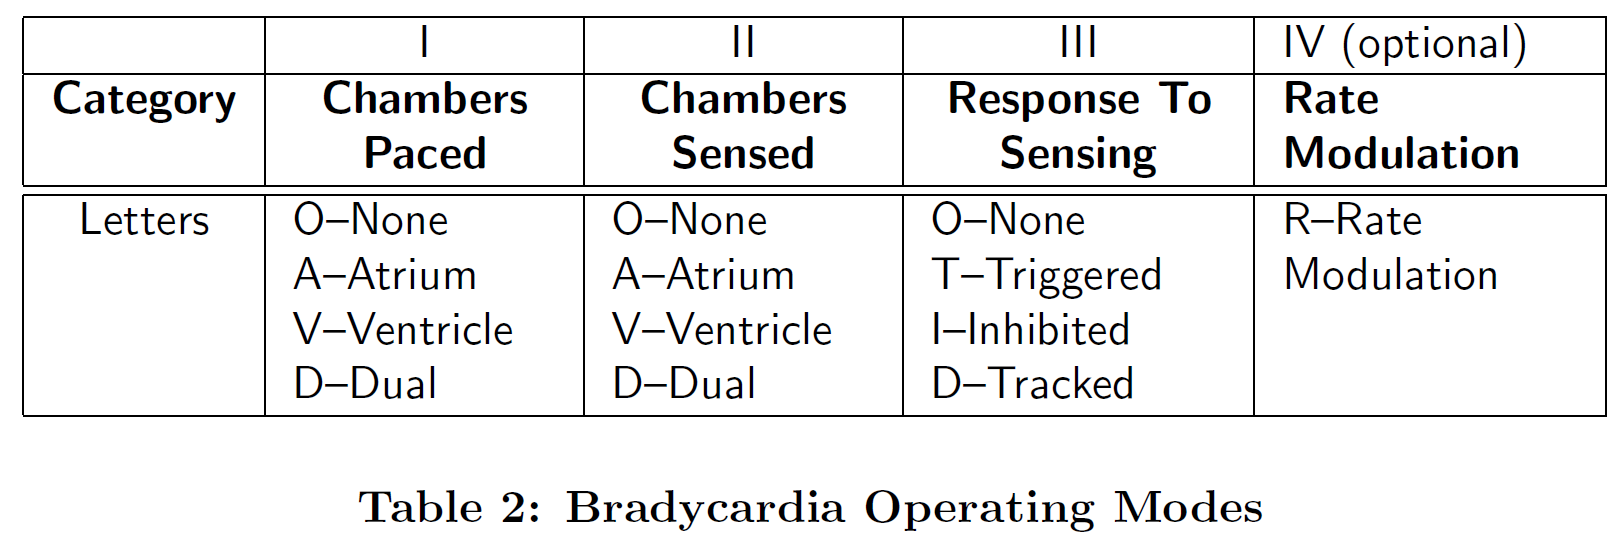
\includegraphics[width=\textwidth]{Operating_modes.png}
	\caption{Intended operation modes for the pacemaker system.}
	\label{fig:Operating_modes}
\end{figure}

\begin{figure}
	\centering
	\includesvg[width=\textwidth]{pg_device_UCD}
	\caption{Use Case Diagram for the PG device based on the original pacemaker specification enhanced with information from the goal diagram knowledge capture.}
	\label{fig:pg_device_UCD}
\end{figure}

In figure~\ref{fig:pg_device_UCD} we have created another UCD enhanced by the knowledge gained from the goal diagram. We identified an additional actor that has use cases; the nurse. The nurse is never explicitly stated as an actor when using the PG device in the original specification. In our goal diagram we have identified that there is a lot of overlap between the nurse and the doctor stakeholders. Aside from programming the pacemaker, which has been explicitly stated in the specification to be done by the doctor, the nurse also has their unique task of patient follow-up that requires they be able to access the historic and diagnostic data from the patient. 

\begin{figure}
	\centering
	\includesvg[width=\textwidth]{DCM_UCD_original_spec}
	\caption{Use Case Diagram for the DCM based on the original pacemaker specification. This diagram combines the hardware and software sub-systems into a single boundary.}
	\label{fig:DCM_UCD_original_spec}
\end{figure}

Next we see in figure~\ref{fig:DCM_UCD_original_spec} a possible interpretation of the information in the DCM overview in a UCD. While the original specification does specify that the DCM sub-system is further decomposed into a hardware platform and software application, it does not make a distinction between the two when specifying the use cases. In this initial modelling attempt, we try to define the use cases for the DCM with its components combined within the system boundary. We also discovered another new actor when creating this UCD: the Strip Chart Recorder. This actor is related to the singleton use case `output to external strip-chart recorders'. This UCD was particularly challenging to create due to all the conjunctive sentences in the specified features. In particular, the `Acquire and show diagnostics (history) and lead signal measurement information' use case is difficult to fully capture who this use case is for. The language used is confusing as by using the word diagnostics the statement seems like this feature is for the Technician. However, because it then specifies history in brackets, similar to what is specified in the `Acquire and show sensor history and trending information' use case, we ultimately decided it is more likely to be used by the doctor and nurse actors. Interestingly, likely due to the overlap between the two stakeholders, the doctor and nurse actors in this model are associated to all the same use cases. As this is supported by their overlapping goals we have a stronger confidence in the correctness of this model.

The DCM system is more challenging to have confidence in the UCD due to the combined nature of the hardware and software sub-systems specified in the requirements. They are heavily coupled which makes identifying what is a software use case and what is a hardware use case difficult as they are currently written. More information may come to light during the refinement however at this point in development it is difficult to gain more insight into how the sub-systems could be decoupled.

\begin{figure}
	\centering
	\includesvg[scale=0.7]{Leads_UCD_original_spec}
	\caption{Use Case Diagram for the leads based on the original pacemaker specification.}
	\label{fig:Leads_UCD_original_spec}
\end{figure}

The leads sub-system is relatively straightforward to model given the limited use cases that were identified. It identified two actors that will use it, the patient and the PG device. However, we have included the DCM as an actor for this system as well. We justify this due to the fact that the DCM being the interface that allows human actors like the doctor or nurse to program or interrogate the pacemaker. 

Overall the exercise of creating the UCDs for the pacemaker has given us a lot of insight that would have otherwise been overlooked using just the original specification. We have identified potentially reusable parts of the system in the rate adaptive pacing. We have identified additional actors that were otherwise implied or overlooked in the original specification. We have discovered potential pain points in the high coupling of the DCM sub-systems. Finally we have identified interactions between the various components of the pacemaker system overall. We also noticed during this process that there is a lot of interpretation involved when creating the models. This can introduce issues in consistency as the results are heavily reliant on the knowledge and experience of the engineers executing this process. 

\section{Product Family Development}

\begin{figure}
	\centering
	
\includegraphics[angle=90, height=\textheight]{pacemaker_fm.png}
	\caption{Feature model based on the UCD for the \pgd.}
	\label{fig:pacemaker_fm}
\end{figure}

One of the benefits of this methodology becomes apparent at this stage of development. Leveraging the equivalency definition we have between use cases and features, all of the use cases that we used in our UCDs are also the features that we will use in our feature models. In figure~\ref{fig:pacemaker_fm} we show a potential product family based on the UCD for the \pgd. We say potential due to the possibility of variability in how engineers can interpret the information from the UCD and goal diagram to create the feature model. For example, single and dual chamber pacing appears twice within the product family due to the necessity to have both rate-adaptive and non-rate-adaptive pacing. There is overlap between the two features, but we put the rate-adaptive versions of the pacing under that feature and the non-rate-adaptive pacing on another level of the model.

Based on the UCD for the \pgd, every use case is necessary for the system, and we identified the reuse of single and dual pacing between rate-adaptive modes. As a result, there is no potential for variability in the final product since all the features are mandatory to complete the system. This provides a starting point for developing the product. We do not take this model as complete as we expect to learn more about the system through the requirement refinement process. As we refine the model this present opportunities for iteration between the phases of this approach. As more features are identified, there can be benefits in iterating between the feature model and \ac{UCD} to explore how they relate to the actors and to other features in the system.

%The refinement process will allow us to iterate and increment on this model.

\subsection{Composition}

Due to the current definition of the metamodel for \tool, feature composition is slightly different. Since we state that all requirements are scoped by their owned features, we do not support cross cutting requirements at this time. When a feature composition is required to define a product based on the feature model, it becomes more of a checklist rather than more traditional composition weaving. This is by design as we want each feature to be self contained with respect to their requirements. This does not exclude dependencies between features however. The validation of feature dependencies can still happen during the composition process if properly implemented. At this time, feature composition is not an automated process in \tool. It requires manual intervention by the user to select what features from the product family to add to a product variant they define.

\section{Requirement Engineering and Refinement}

With a prototype product family created from the UCD, we can start to explore the use cases and refining them towards more proper requirements. We do this by taking the use cases and refining them as a user story. We use the following structure when refining a use case to a user story:

\begin{itemize}
	\item \textbf{Use case}: Provide programmable pacing
	\item \textbf{Actor}: Doctor, DCM
	\item \textbf{Precondition}: Pacemaker \pgd\ is active and can connect to the DCM.
	\item \textbf{Trigger}: Doctor wants to program pacemaker to mitigate patient bradycardia symptoms via DCM interface.
	\item \textbf{Success Scenario}:
	\begin{enumerate}
		\item Doctor accesses \pgd\ via DCM.
		\item Doctor verifies they are connected to correct \pgd.
		\item Doctor selects the desired pacing operation mode.
		\item Doctor sets the various parameters based on the chosen pacing operation mode (pace pulse characteristics, rate sensing settings, delays etc).
		\item Doctor pushes programmed mode and parameters to the \pgd.
		\item Doctor disconnects DCM from \pgd.
		\item Doctor logs off from DCM.
	\end{enumerate}
	\item \textbf{Secondary Scenarios}:
	\begin{itemize}
		\item Doctor connects to the wrong \pgd\ via DCM.
		\item Doctor makes a mistake programming the \pgd\ via DCM.
		\item Communication fails or is interrupted during push from DCM to \pgd.
		\item Doctor is unable to access the \pgd\ via DCM.
	\end{itemize}
	\item \textbf{Success Postcondition}: \pgd\ is correctly programmed and pacing the patients heart correctly and safely.
\end{itemize}

The steps outlined in the success scenario are the functional requirements for the use case. They outline what needs to happen for the actor to accomplish whatever task is outlined. The outcomes in the secondary scenarios provide alternative results of actors actions. These alternative outcomes can be safety hazards, security hazards, system malfunctions, or user errors. The secondary scenarios outline the justifications for mitigating requirements in order to improve the chance that the actor will arrive to the success postcondition, in this case that the \pgd\ is correctly programmed and pacing the patients heart correctly and safely. In the context of our methodology, mitigating requirements are most commonly categorized into safety, constraint, or qualitative requirements. At this time we have not ruled out that a mitigating requirement may lead to a functional requirement, however based on our experiences we support the convention that they are a better fit for the non-functional requirement types.

With these requirements identified, we can begin modelling them in the requirement canvas. In \tool, the requirement canvas is embedded in the features of the product family. This is the feature-requirement encapsulation that we outlined in the methodology. In figure~\ref{fig:req_canvas_creation_UI}, we show how a user can create an embedded requirement canvas.

%The mitigating requirement can be safety, constraint, or qualitative requirements. While we cannot declare that none of the secondary scenarios could lead to a functional requirement, by convention it is best to attempt to classify them in one of the non-functional types first. 


%The scenarios outlined in the secondary scenario section are specify alternative outcomes that can represent alternative outcomes for the actor. 

\begin{figure}
	\centering
	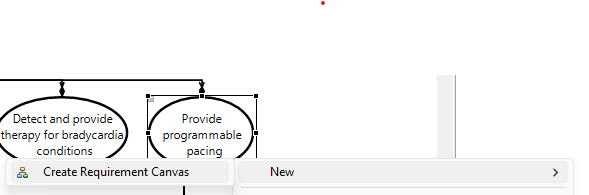
\includegraphics[width=\textwidth]{req_canvas_creation_UI.png}
	\caption{When right-clicking on a feature, a context menu appears allowing users to create a requirement canvas that is embedded in the selected feature.}
	\label{fig:req_canvas_creation_UI}
\end{figure}

\begin{figure}
	\centering
	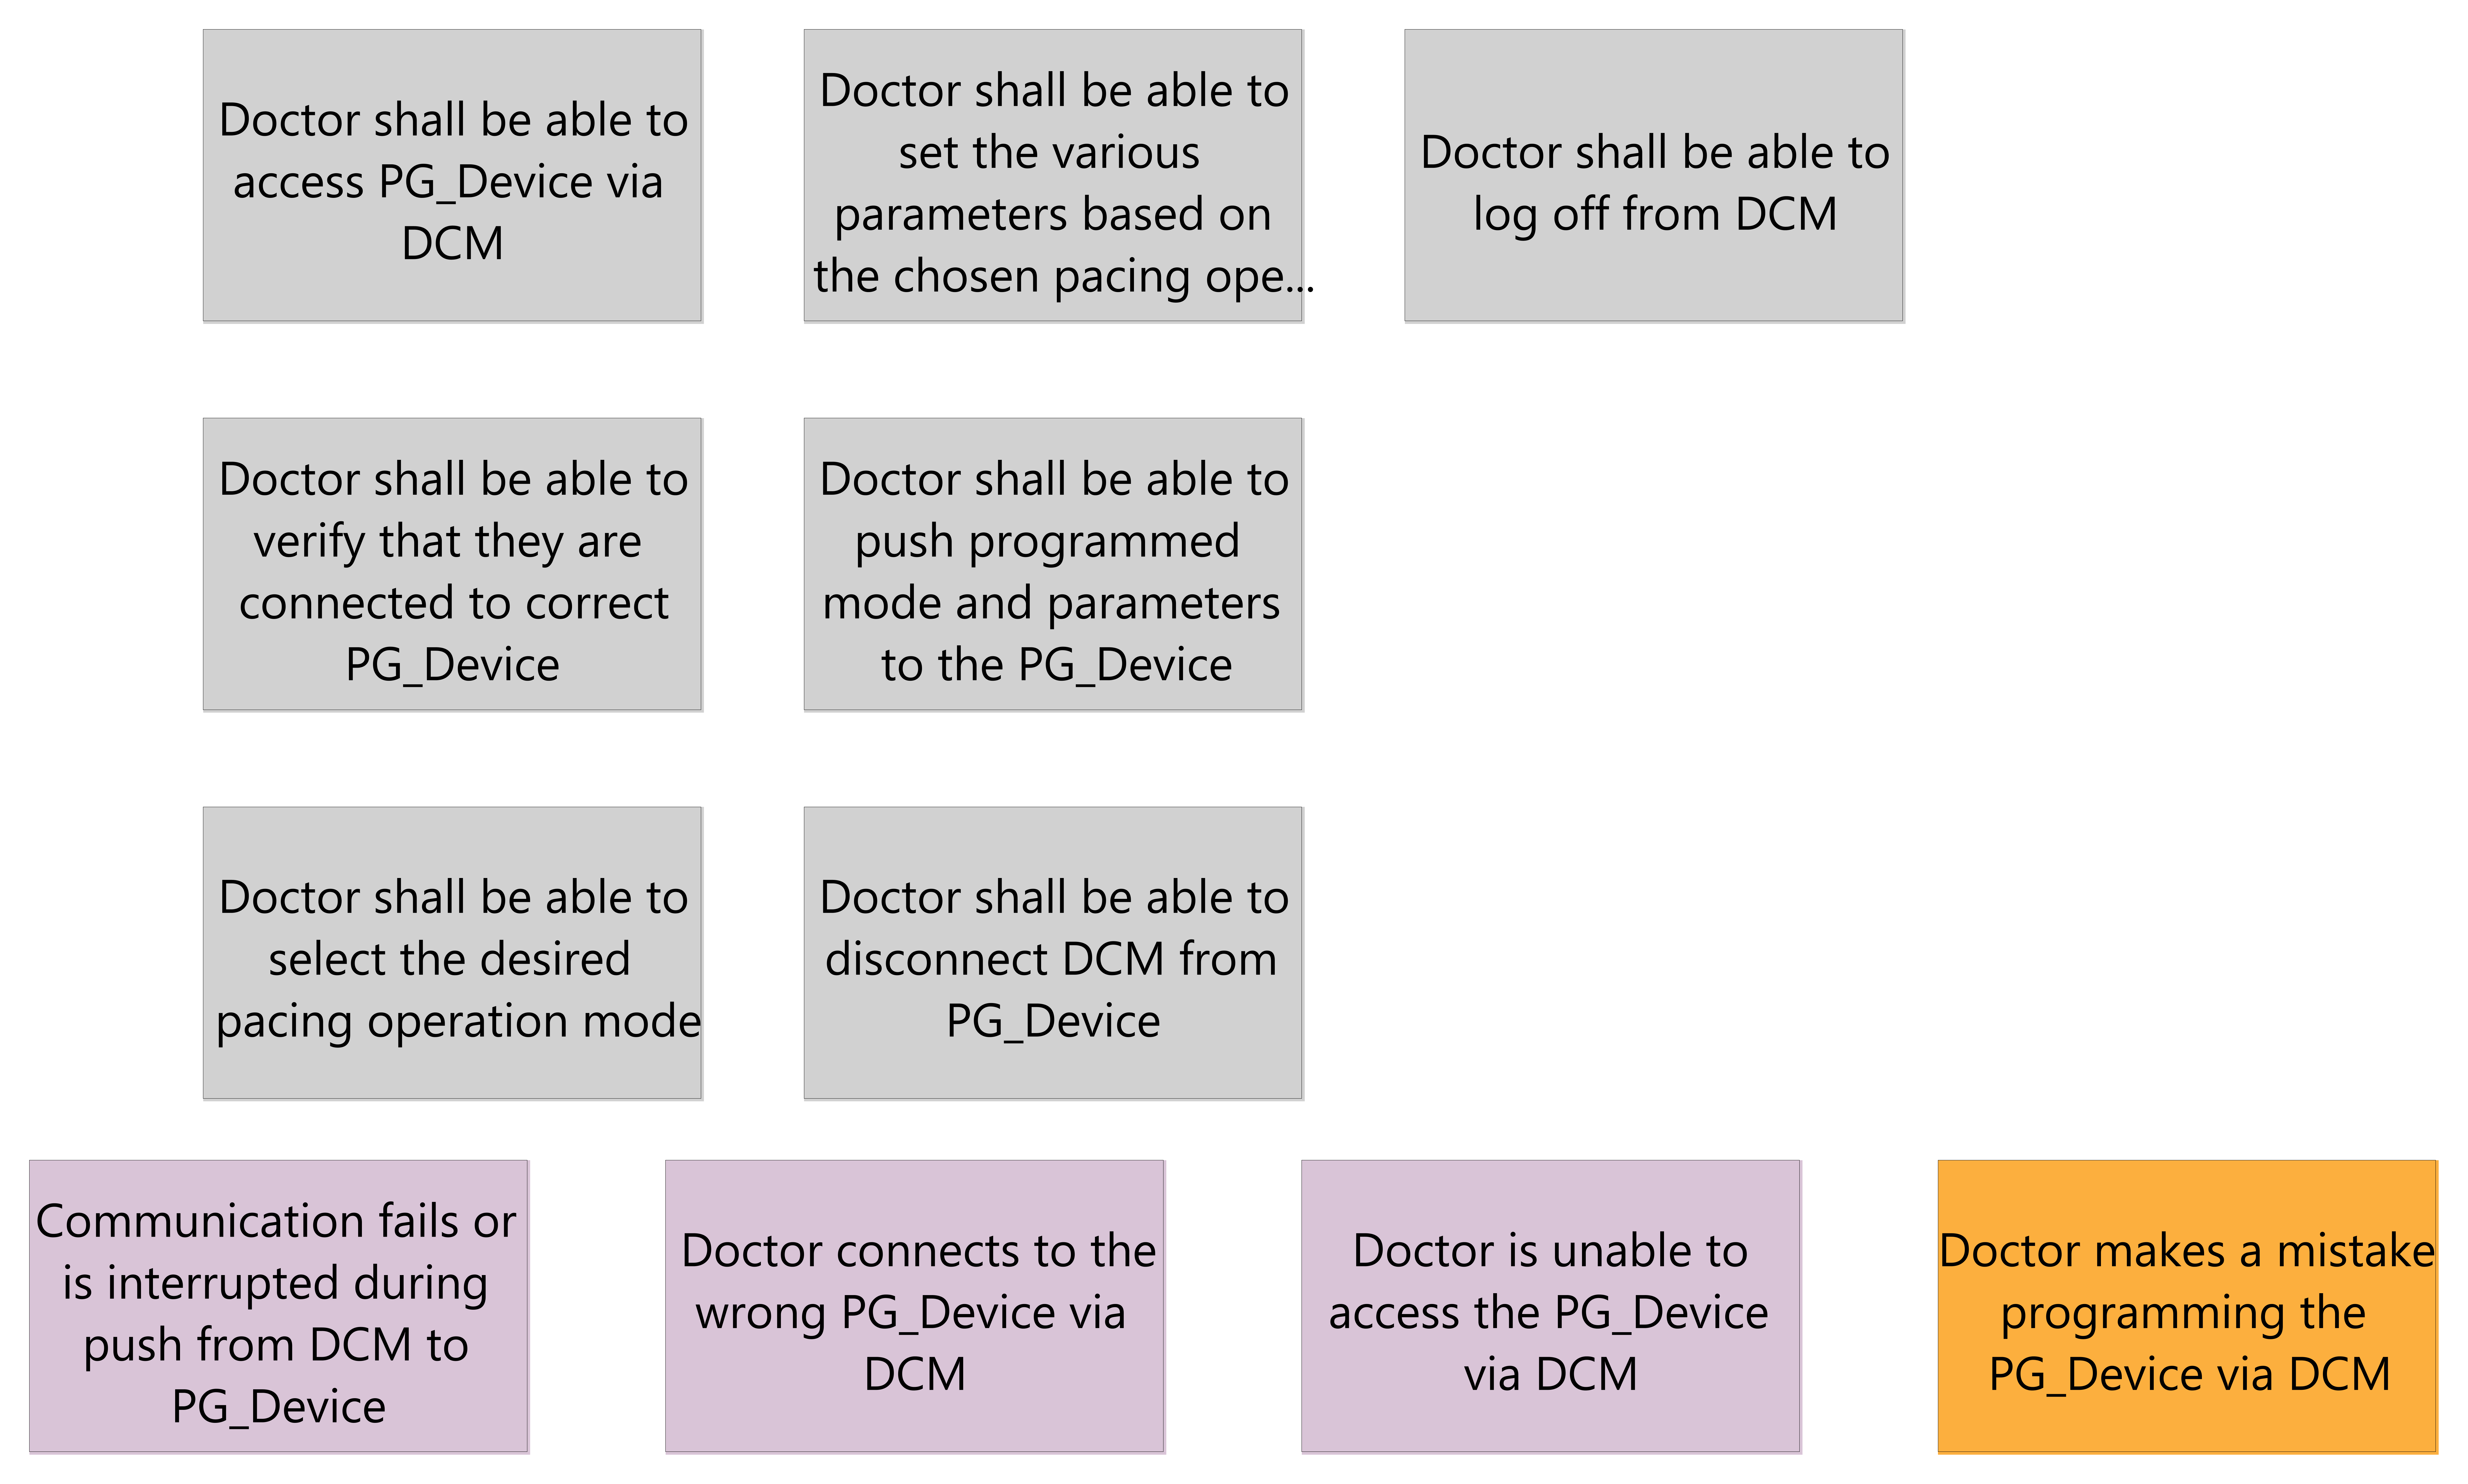
\includegraphics[width=\textwidth]{pacing_reqs.png}
	\caption{Requirements for the `Provide programmable pacing' use case.}
	\label{fig:pacing_reqs}
\end{figure}

In figure~\ref{fig:pacing_reqs} we show all the requirements created in the model as previously identified to match the refinement of the user story. In figure~\ref{fig:req1_spec}, figure~\ref{fig:req2_spec}, and figure~\ref{fig:req3_spec} we also show the Gherkin specifications for the expected behavior of the first three requirements.

\begin{figure}
	\begin{lstlisting}
		Given{
			Precond one: "The pacemaker PG_Device is active and can connect to the DCM"
		}
		When{
			Event one: "Doctor wants to program pacemaker to mitigate patient bradycardia symptoms via DCM interface"
			Event two: "The doctor attempts to access the PG_Device via DCM"
		}
		Then{
			Postcond one: "The doctor is able to connect to a PG_Device"
		}
	\end{lstlisting}
	\caption{Gherkin specification for the first requirement of the \pgd.}
	\label{fig:req1_spec}
\end{figure}

\begin{figure}
	\begin{lstlisting}
		Given{
			Precond one: "The doctor is able to connect to a PG_Device"
		}
		When{
			Event one: "The doctor wants to verify they are connected to the correct device"
		}
		Then{
			Postcond one: "The PG_Device shall communicate to doctor via DCM identification to allow doctor to verify device identity"
		}
	\end{lstlisting}
	\caption{Gherkin specification for the second requirement of the \pgd.}
	\label{fig:req2_spec}
\end{figure}

\begin{figure}
	\begin{lstlisting}
		Given{
			Precond one: "The doctor has verified they are connected to the correct device"
		}
		When{
			Event one: "The doctor wants to change or select the desired pacing mode"
		}
		Then{
			Postcond one: "The doctor shall be able to select from the available pacing options"
		}
	\end{lstlisting}
	\caption{Gherkin specification for the third requirement of the \pgd.}
	\label{fig:req3_spec}
\end{figure}

The requirement entities in the canvas have facilities that allow us to specify our requirements in greater details. Due to the user stories that we used to refine the use cases into the requirements necessary to satisfy the successful postcondition, there is an implied ordering that is generated for the functional requirements. We can see this ordering reflected in the Gherkin specifications. The postconditions for one requirement often be reused as the preconditions for the next. The tool does not make this relationship explicit, but the specification does allow for it. This provides some flexibility to the engineers using this methodology for how they want to specify relationships between their requirements. 

Another benefit of these ordered requirements is that it can help with planning feature development. Engineers can identify dependencies between requirements within a feature more easily and plan what stages of development need to be completed sequentially and which ones can happen in parallel. This lends confidence to the claim of this methodology helping with FDD. The feature becomes well defined by the requirements, each requirement has the opportunity to be well specified by the engineers, and plans can be made to tackle the order of development to complete the feature. This includes the satisfaction of functional, qualitative, constraint, and safety requirements alike.

Another part of the requirement canvas is the ability to assign test cases and reviewers to specified requirements. At this point in development, the purpose of those model elements is primarily bookkeeping. A further benefit of using the Gherkin syntax are the many existing libraries that support it testing. At this time, we do not natively support testing in the tool. We do however, want to be able to keep track of which requirements have been satisfied and which ones have not. Additionally, we also want to keep track of which ones have been reviewed and approved. As part of the requirement engineering process it is important to keep track of which requirements are ready to development, and which ones are still undergoing refinement. We show how this can appear for the pacemaker in figure~\ref{fig:pacing_reqs_tests_reviews_export}. Naturally, once these model elements are added and connected to requirements, they are automatically updated in the traceability matrix as well.

%\begin{figure}
%	\centering
%	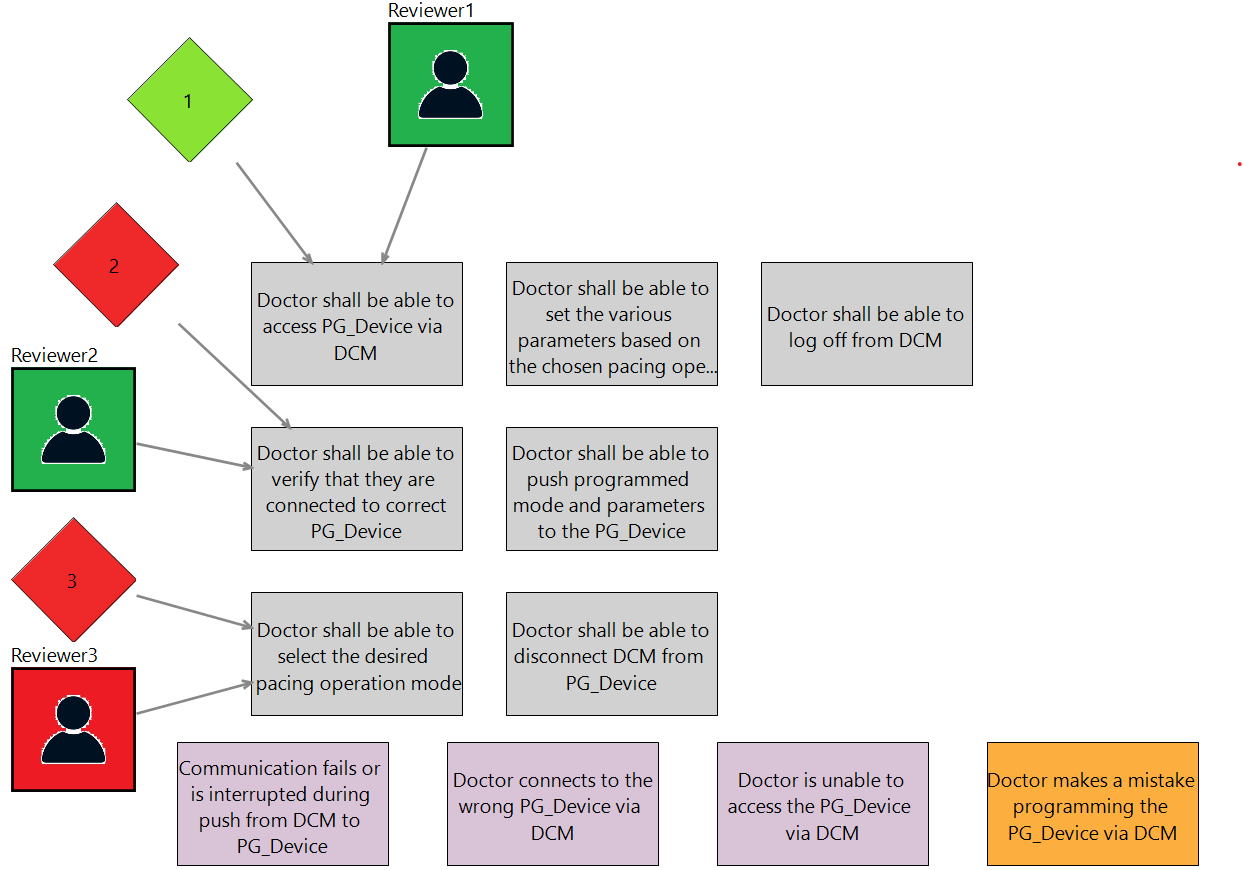
\includegraphics[width=\textwidth]{pacing_reqs_tests_reviews.png}
%	\caption{Requirements for the `Provide programmable pacing' use case.}
%	\label{fig:pacing_reqs_tests_reviews}
%\end{figure}

\begin{figure}
	\centering
	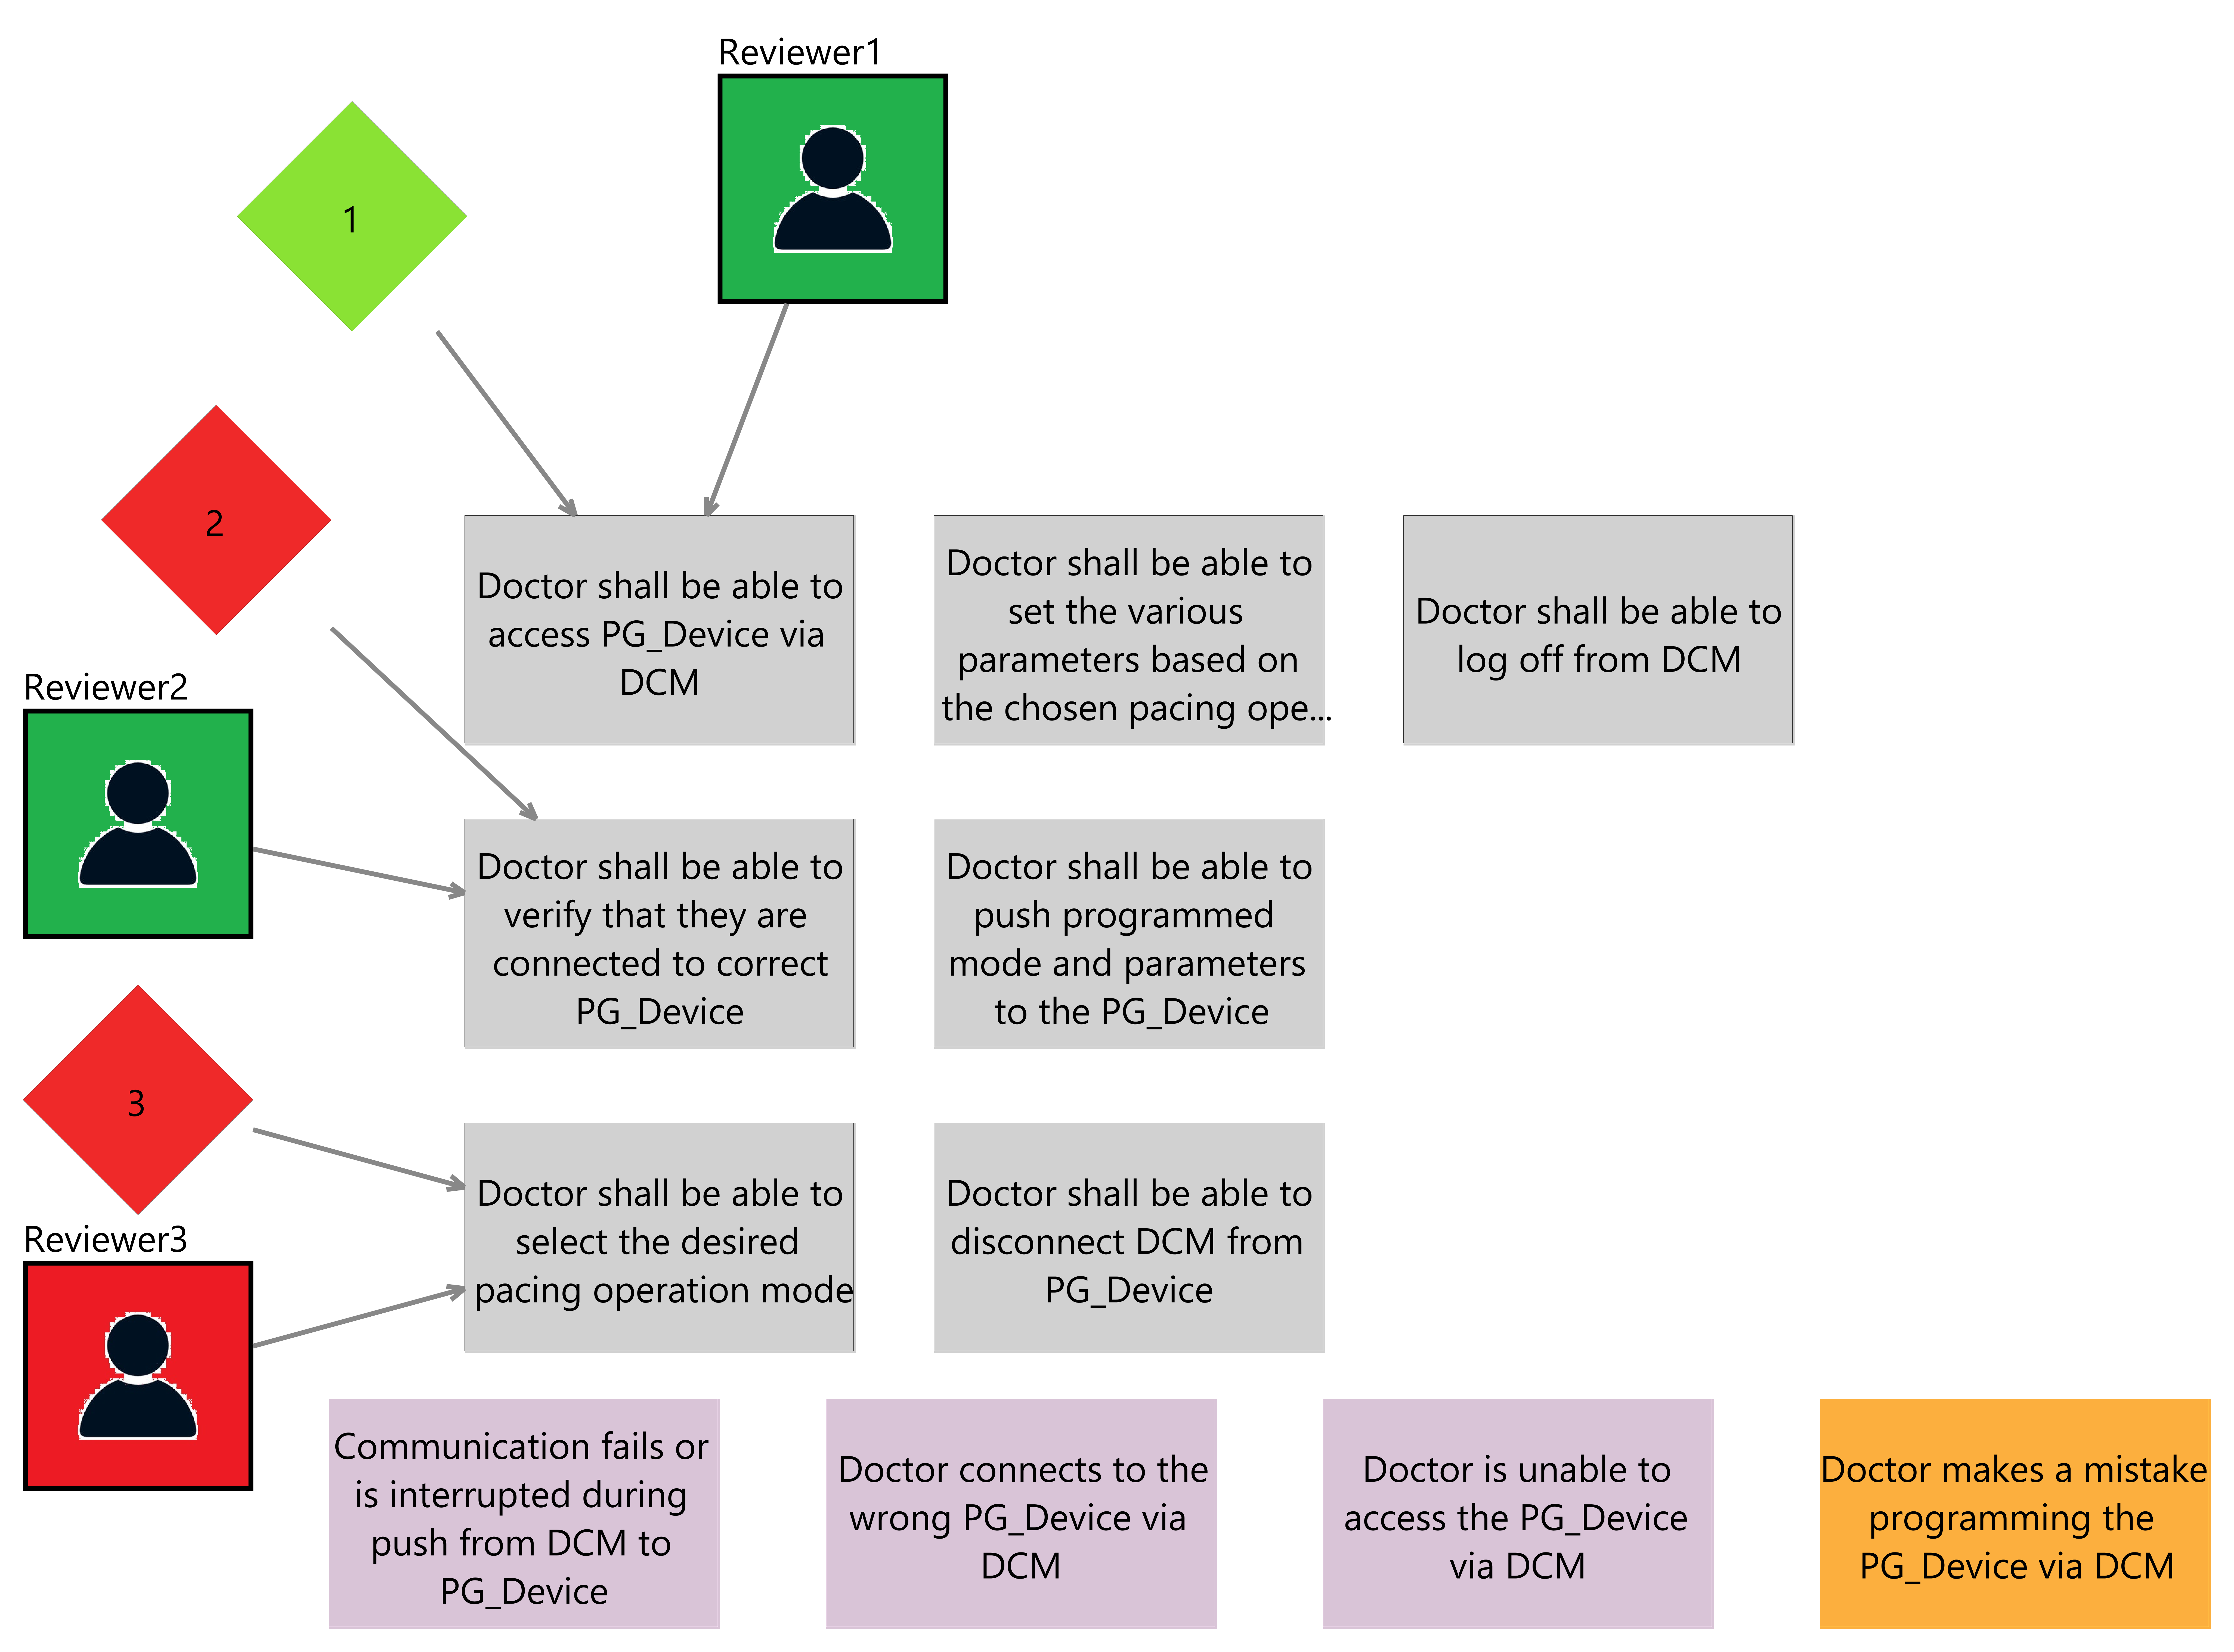
\includegraphics[width=\textwidth]{pacing_reqs_tests_reviews_export.png}
	\caption{Various stages of approval and testing for the requirements.}
	\label{fig:pacing_reqs_tests_reviews_export}
\end{figure}

\begin{figure}
	\centering
	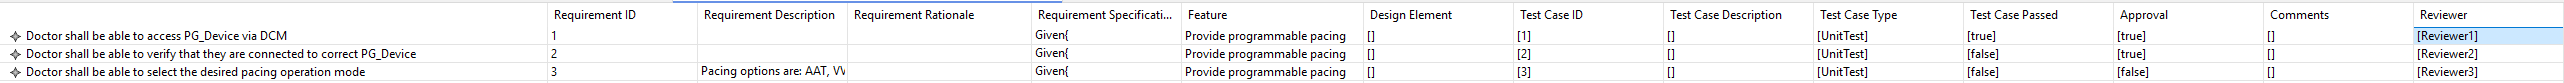
\includegraphics[width=\textwidth]{pacing_reqs_tests_reviews_trace.png}
	\caption{Showing how traceability is automatically maintained throughout requirement approval and testing.}
	\label{fig:pacing_reqs_tests_reviews_trace}
\end{figure}

At this stage we have created a functional behavioural specification for the ``Provide programmable pacing'' use case beyond what is in the original specification. We have justified our requirements using the use cases from the \ac{UCD} which are in turn supported by our goal diagrams. We have also identified qualitative and safety requirements that were not identified in the original specification. We have demonstrated flexibility in how we can specify these requirements using the Gherkin syntax. This has shown the benefit of a semi-formal approach as we can get an order to our functional requirements if desired to help with project planning and scoping. This also shows potential integration points with existing \ac{FDD} development methods. The natural language also makes the specification process relatively easy to learn and approach while allowing meaningful specifications to help development. Finally, we have shown that all of these efforts automatically create a traceability matrix for us with no extra steps or inputs by us during this process execution.

\section{Iterations and Incrementation}

For the purpose of this methodology, iterative changes are thought of as cycles between development phases (features and requirements, requirements and design, design and implementation). The idea for this definition is that there are lessons learned when working through a subsequent development phase that can inform and create cause for repeating a process from a previous phase. In the case of this methodology, if there is a need identified during the requirement phase, it may create a cause for repeating one of the processes in feature modelling phase. 

Incremental changes are thought of as changes within a single development phase. Currently, \tool\ supports maintenance of the traceability matrices through incremental changes as we have defined them. As engineers work through the various steps within a development phase, they will be constantly adding, modifying, or removing artifacts until they reach a satisfactory result. We consider all of these incremental changes until they get enough completed to move onto the next phase of development.

There are three traceability matrices that are supported in \tool; project traceability, feature-feature traceability, and feature-requirement traceability. Project traceability and feature-requirement traceability are defined to focus on traceability of the requirement entities. Project traceability is the traceability matrix for the entire project. Feature-requirement traceability is a traceability matrix that is scoped to a single feature. The Feature-feature traceability matrix is a tabular representation of the feature model that is defined within the project.

These are a second syntactic representation of the modelling environments present within the tool. Since they are semantically equivalent, any change to the requirements in the requirement canvas or features in the feature modelling environment are automatically reflected in their respective traceability matrix. The tabular environments, though somewhat limited, are also capable of defining new requirements. The limitations are that test cases and reviewers cannot be created in the tabular environment. This is by design as it forces users to manually create those traces explicit in the modelling environment and reflect on what test cases are being created and who is approving of the requirements.

We currently have limited support for iterative changes according to our definition. While changes that are made to an existing model will naturally be automatically reflected in the traceability matrices, the impact of the change cannot currently be assessed. Based on the metamodel for \tool, however, the mechanisms to support change impact analysis are all present. This is due to the nature of traceability that is inherently built into the model and the way we require explicit connections between elements in order for a model to be what is consider syntactically valid by our current conventions. 

\tool\ is also currently only scoped to feature and requirement modelling. It does not currently support \ac{UCD}s or goal diagrams within itself. As a result, we do not automatically generate and maintain traceability to those phases of development. By having all the modelling environments connected within \tool, we will have more confidence in being able to trace iterative changes and change impact more comprehensively through the various stages of development. 

%\subsection{Coherence in Medical Device Development}
%
%\subsection{Relevance in Medical Device Development}
%
%\subsection{Impact in Medical Device Development}
%
%\subsection{Efficiency in Medical Device Development}
%
%\subsection{Effectiveness in Medical Device Development}
	\chapter{Future Work}

While the results of our proposed methodology and tooling are promising, there are some definite short-comings at present. While CyclicL is self-contained with regards to features and requirements, there is no traceability between the \ac{UCD} and goal diagram to the tool. This presents challenges to comprehensive traceability from requirements through the features to their sources. This also causes a gap in analysis when performing iterative changes as there are no facilities currently that can enable change impact analysis between feature modelling and the \ac{UCD}. As users learn more about their product we anticipate and encourage them to iterate through the various phases of development in this methodology and we want to support that computationally as well.

Using this methodology to support safety and security assurance case development is another avenue we would like to explore. As this methodology highly emphasizes traceability, there could be opportunities for supporting assurance case development. This possibility is part of the reason for the ``Safety'' type for the requirement canvas. This would include the traceability to the \ac{UCD}s and goal diagrams in \tool.

%This presents another challenge of traceability and justification. It requires the engineer to be aware of the links between the domain and problem space analysis and the feature and requirement models in the tool. This implicit knowledge will eventually need to be documented somewhere to support both future development changes and assurance for safety-critical development. As a result, one potential path is creating a bridge between the domain analysis modelling and the current tool to extend the traceability all the way up to the concept phase of development. While we expect \ac{UCD} and goal diagrams to remain mostly static once they are created, the direct traceability could be helpful documentation for onboarding new employees to help them get familiar with why certain decisions were made, support change impact analysis justifications, and aid the development of assurance case by having complete end-to-end traceability between the problem space and the solution space.

The implementation of the tool, \tool, is still incomplete as we have only demonstrated the capability of the minimum viable product. There are many functions we will need to add to have a more complete tool. There are currently no constraints in the tool to ensure that all user created models are valid according to the metamodel. Thus, there is no way to validation tools to ensure that the engineering artifacts created are semantically or syntactically meaningful, useful, or computable.

Thus there is potential for users to create semantically meaningless models even if the syntax is shown as correct. We are currently relying on conventions and good engineering to create semantically meaningful models but this is very difficult to maintain at scale within a company or industry. Another lane of development would be in allowing users to create these models textually as well as graphically. Very often adoptability of a tool, especially an \ac{MDE} tool is difficult as many engineers are unfamiliar with \ac{MDE} techniques and approaches. Creating a textual environment for creating these models may help with usability and approachability of CyclicL for use in industry. Next, we would want to implement a method of consistency checking within the tool. This would remove a lot of the burden from the engineer to ensure that their features are consistent and their requirement are consistent between features. This is a unique challenge as the requirements are specified using the Gherkin behavioural approach and thus may require us to re-evaluate what type of specification language we implement within the requirement canvases of CyclicL.

Other future work tasks that have been mentioned throughout this thesis include integration with existing test compilers, integration with previous feature modelling tools, and general UI enhancements. As there are many Gherkin test environments, building a bridge to allow integration with \tool\ would be helpful to verification tracking and traceability. Integration with another feature modelling tool, such as FeatureIDE, would be serve as an exploration for the impact of the feature-requirement hierarchy defined in this thesis on existing feature weaving and composition techniques.



	\chapter{Conclusion}


What comes first, the requirement or the feature? In this thesis we have attempted to outline an answer to this question. incidentally, and perhaps unsurprisingly, the answer is both and it depends. Both realities are possibilities for companies in industry as they startup new product development from scratch or try to reuse previous work for a new model. So we support both of them. 

The ultimate answer however, is neither. The stakeholder use cases and goals come first as we conduct a domain analysis and problem space exploration. We have shown that following Meyer's requirements engineering approach we can leverage both informal and formal \ac{MDE} techniques to perform a domain and problem space analysis. We found that goal diagrams were an easy to use, informal approach to capturing knowledge of what stakeholders really want to do which helped to inform why they would want to use a product we develop. The \ac{UCD} was important for establishing how the would use our product. Identifying what interfaces the stakeholders would need from the product to accomplish their goals. Goal diagrams and \ac{UCD}s formed the core of our informal modelling techniques for domain analysis and problem space exploration.

Feature modelling and our requirement canvas leveraged more formal approaches to modelling and problem space exploration as with \tool\ we could enforce syntactic and semantic rules when creating the models. Equating features and use cases also helped to establish requirements for our features as we refined the use cases into user stories. With our proposed feature-requirement hierarchy, those requirements are immediately scoped and owned by the features making an easy transition from problem space exploration to requirement specification. We have demonstrated both formal and informal approaches to domain analysis, problem space exploration, and requirement development while using \ac{MDE} techniques. We have explored several processes for accomplishing these tasks in multiple environments. Finally, we have demonstrated how this methodology can be used to identify gaps in existing documentation and how to improve requirements specification and identification. Thus, we conclude that we have satisfied~\ref{RQ4}

% who our customers/users/stakeholders are, what we expect them to do with our system, and why they would want to use our system to satisfy their goals. We have shown to we can map the identified use cases to features of our system. We have shown how we can derive high-level requirement from our goal diagram and how we can refine and decompose those requirements. Thus we have shown satisfaction of~\ref{RQ4}.



%Thanks to this process contribution, we are also able to identify features and elicit requirements in parallel or in either order. The next step we need to do is decide which features own which requirements. This is first done at a high-level as we map goals to use cases, and then equate use cases to features. Then we can refine those use cases into requirements through user stories that are owned and scoped by the feature to ensure relevance. We have shown an added bonus to this approach in the implicit ordering that emerges in the functional requirements. This implied order has the potential to help with project planning in \ac{FDD} development environment and helps ensure that the features are well defined. This satisfies~\ref{RQ1}.

\ac{FDD} is a well established development strategy. A major contribution of this thesis is the proposed feature-requirement hierarchy that establishes features own their requirements. Another contribution is how we have equated use cases from \ac{UCD}s to features in \ac{PLE}. Our methodology refines the use cases into user stories to create our requirements for each use case. Due to having equated use cases and features, those requirements are thus also applicable to the feature. When combined with the proposed feature-requirement hierarchy we end up with well defined requirements for each feature. An added bonus to this we discovered was a natural ordering that formed in the requirements due to the nature of using user stories as a refinement process. These all contribute to having well defined and scoped features, and potentially aiding in project planning due to the implied ordering of requirements from the user stories. These are all possible ways to enhance \ac{FDD} development environments, satisfying~\ref{RQ1}



%using the feature decomposition in the feature model. This implies a natural decomposition in the requirements as well as they are scoped by the features that own them. Overall, there is a much clearer path to specifying features in a \ac{FDD} environment with the supporting methodology and tool. 

%map which features satisfy a user goal or goals. Then we can refine those goals into requirements that are owned by the feature, all scoped by the feature to ensure relevance. We have shown an added bonus to this approach using the feature decomposition in the feature model. This implies a natural decomposition in the requirements as well as they are scoped by the features that own them. Overall, there is a much clearer path to specifying features in a \ac{FDD} environment with the supporting methodology and tool. This satisfies~\ref{RQ1}.

One of the main contributions of our methodology is the feature-requirement encapsulation. By defining this hierarchy, we have shown how it facilitates traceability between features and requirements. We also removed ambiguity in the relationship between features and requirements. We have demonstrated how this hierarchy enables increased granularity of traceability through our implementation of CyclicL. We were able to define a formal metamodel to capture this hierarchy and implement a tool to show satisfiability of this proposal. Through CyclicL, we exposed the benefit of this hierarchical relationship between features and requirements in the semi-automated maintenance and generation of traceability matrices between features and requirements. This was completed as a by product of following the methodology and naturally using \tool\ to create models and specify our requirements. We thus got the traceability matrices without any manual intervention or extra steps in the engineering process. We conclude that this reduces much of the time and effort that would traditionally have been spent manually creating or maintaining engineering data traceability, satisfying~\ref{RQ2}.

%We can show what features own the requirements. 

Finally, CyclicL has shown the potential benefits of a \ac{PLE} tool that is self contained with requirements as part of the tool in the context of iterative and incremental development. We have shown that we can support incremental development of both feature models and requirement models in CyclicL. By leveraging \ac{EMF} and Sirius, we were able to show the possibilities enabled by a tool that will maintain traceability through both requirement changes and product changes without dependencies on external support. While there are still some limitations in the current tool capabilities to support iterative changes, we have demonstrated how future development can continue to address these short-comings. Due to the currently limitations in the tool, we conclude that we have partially satisfied~\ref{RQ3} with \tool\ as a tool that supports iterative and incremental development of traceability in parallel to feature and requirement development. We give it a partial designation as there are still limitations on how \tool\ can support iterative changes under our current definition of a change between development phases.

Overall our methodology has shown demonstrable improvements on an existing requirement document, provided avenues for potential improvements in requirement engineering and feature modelling, and shown potential for integrating with existing development practice. \tool and its supporting methodology are ripe for further exploration and continued development to support safety-critical development in further domains and potentially as a more generalized approach to requirement engineering across industries.


%---------------------------------------------------------------------
%			Backmatter
%---------------------------------------------------------------------

\begin{appendices}
	\chapter{}

\section{Boston Scientific Pacemaker Requirements}
\label{apdx:Req}
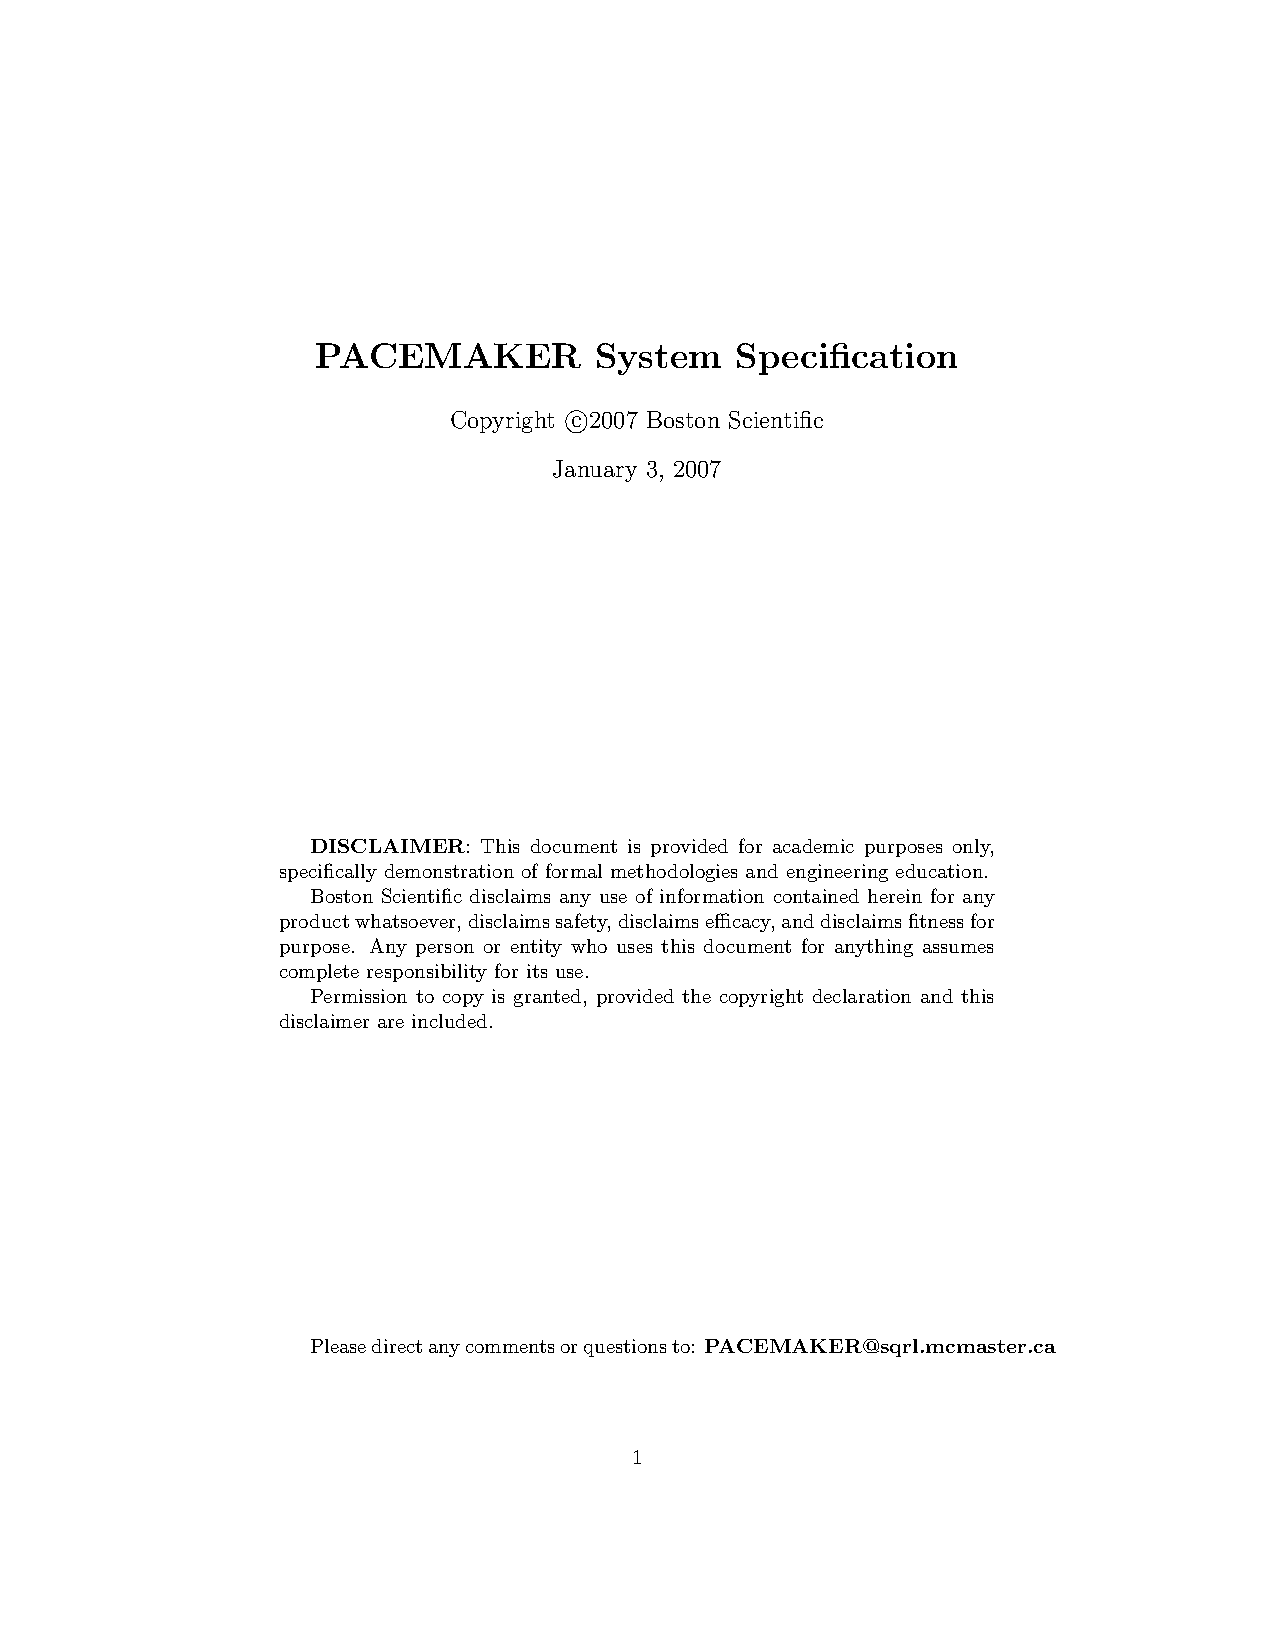
\includepdf[pages=-]{PACEMAKER}

\section{CyclicL Complete Metamodel}
\label{apdx:CyclicL_mm}
\begin{figure}
	\centering
	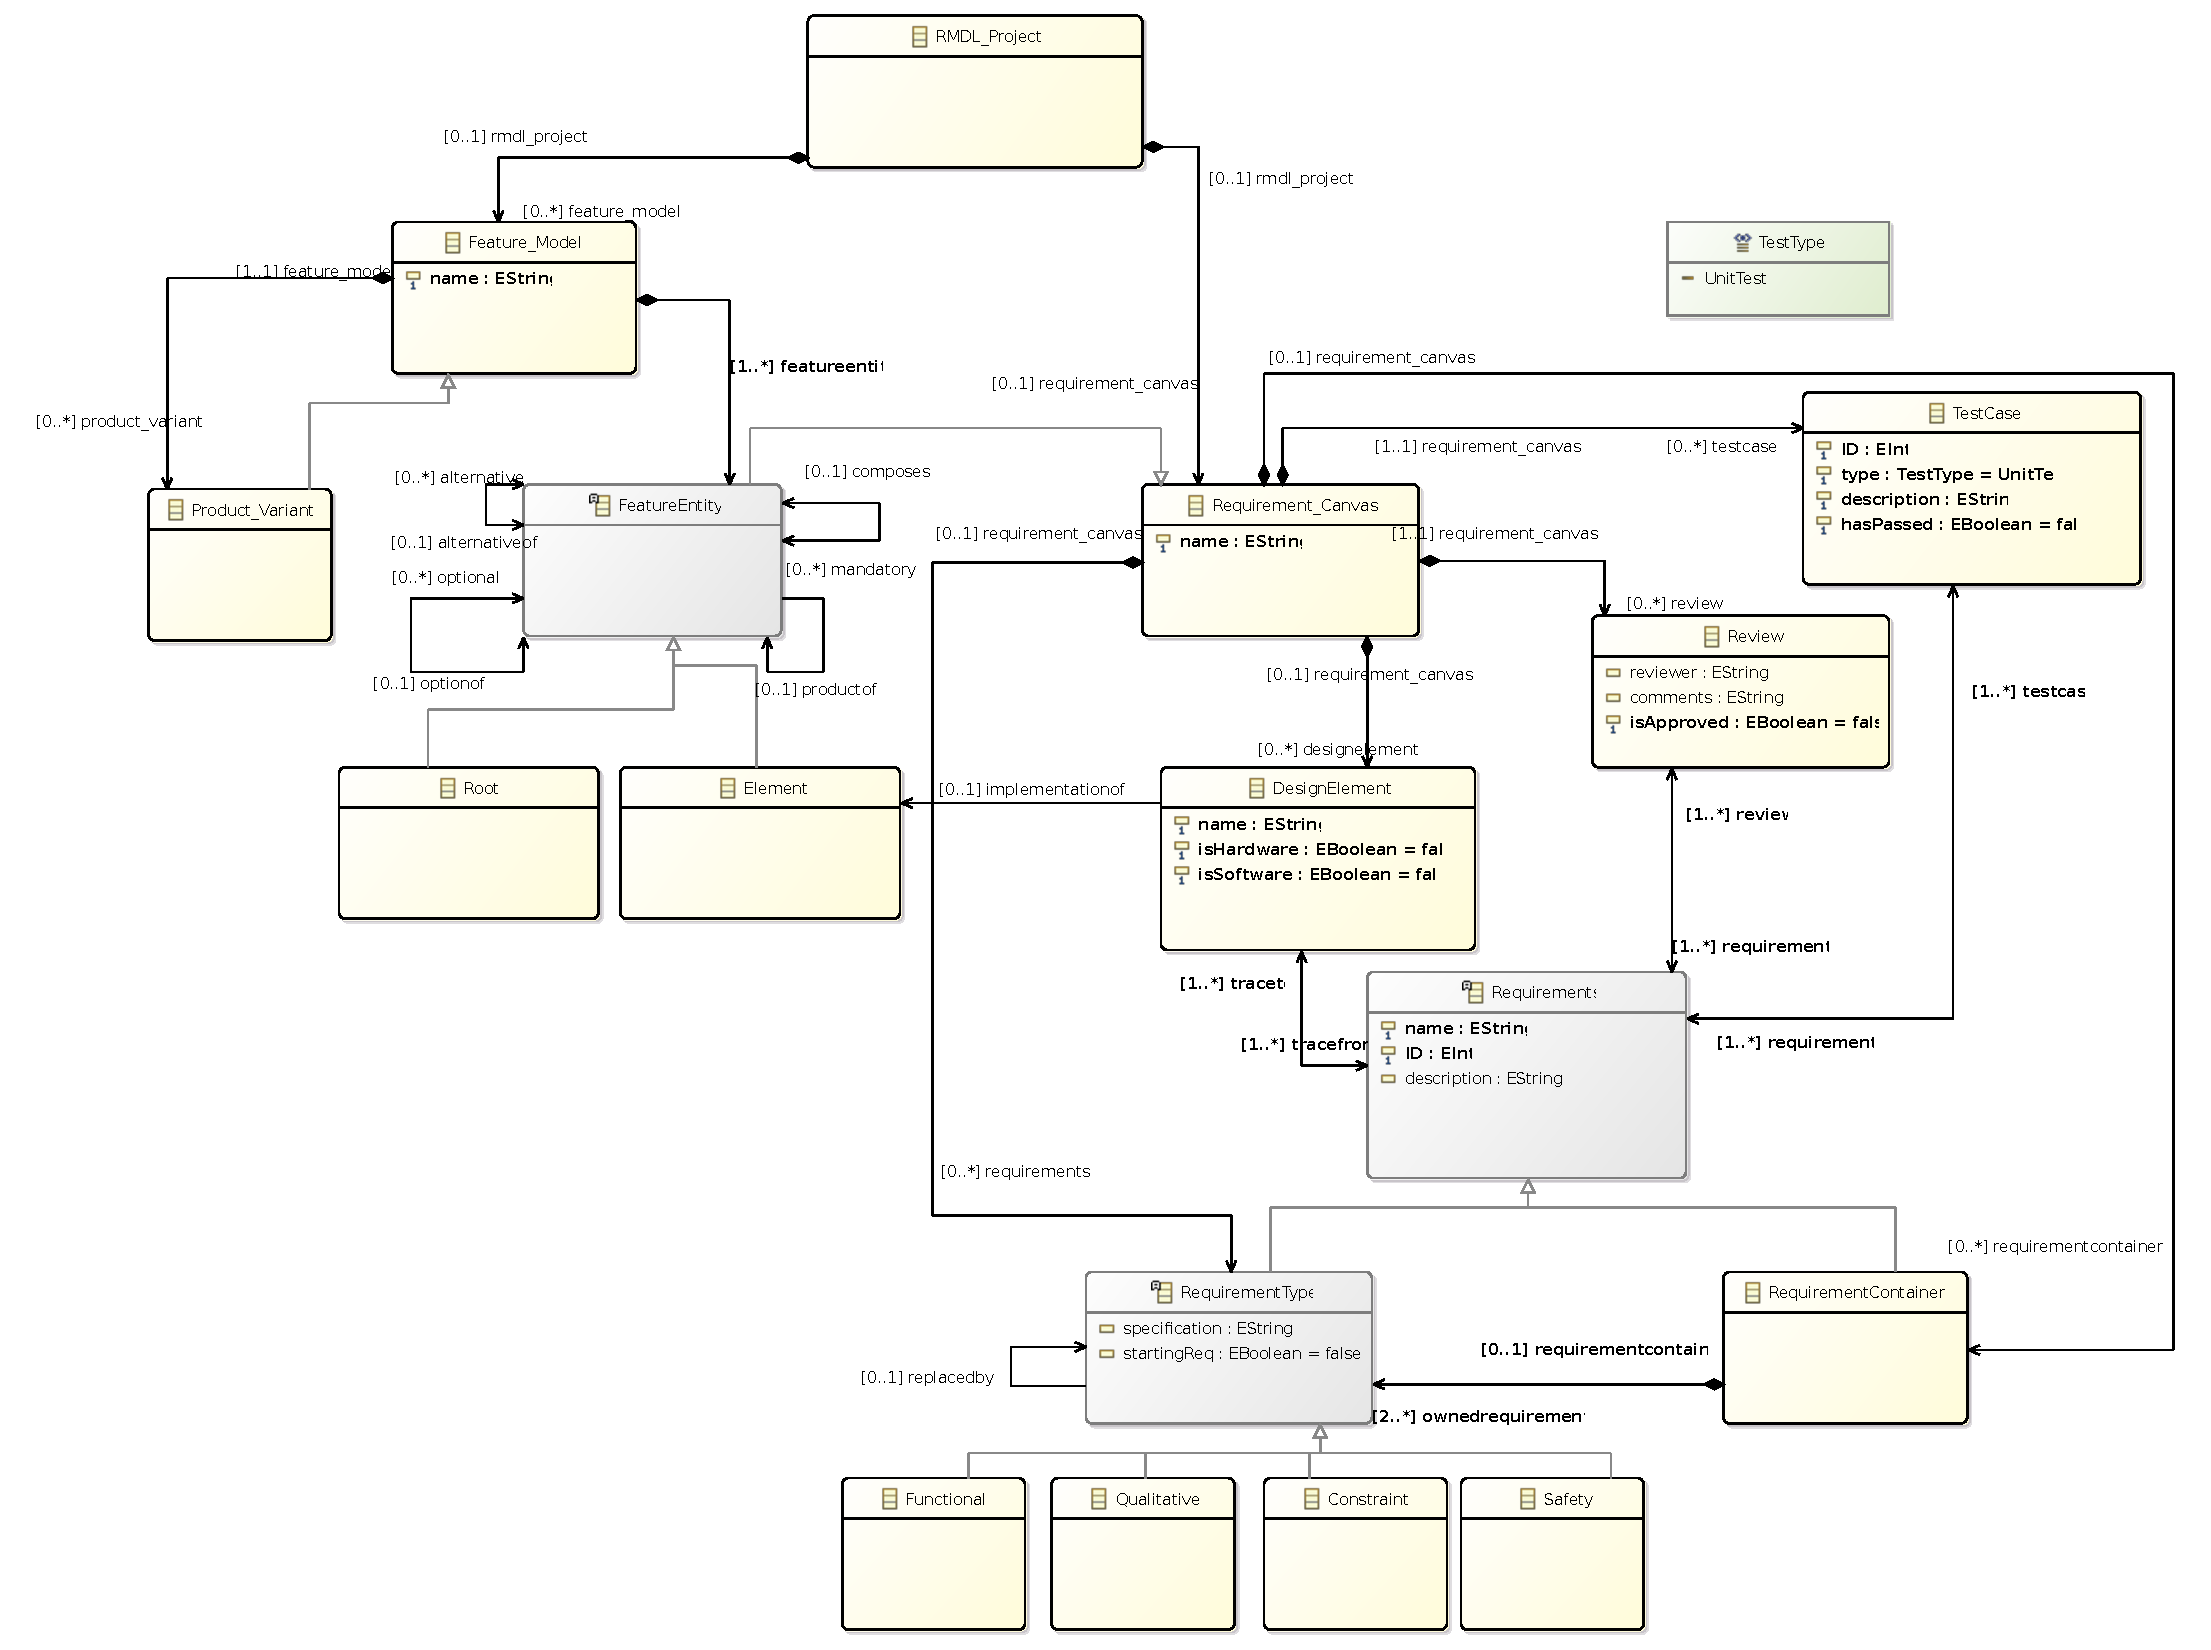
\includegraphics[width=\textwidth]{metamodel.pdf}
	\caption{CyclicL metamodel. Shows the specification for both the requirement canvas and feature modelling portions of CyclicL.}
	\label{fig:metamodel}
\end{figure}
\end{appendices}

\printbibliography
\label{ContentEnd}
\end{document}
%---------------------------------------------------------------------